% Options for packages loaded elsewhere
% Options for packages loaded elsewhere
\PassOptionsToPackage{unicode}{hyperref}
\PassOptionsToPackage{hyphens}{url}
\PassOptionsToPackage{dvipsnames,svgnames,x11names}{xcolor}
%
\documentclass[
  10.5pt,
  a4paper,
  DIV=11,
  numbers=noendperiod]{scrartcl}
\usepackage{xcolor}
\usepackage[margin=24mm]{geometry}
\usepackage{amsmath,amssymb}
\setcounter{secnumdepth}{5}
\usepackage{iftex}
\ifPDFTeX
  \usepackage[T1]{fontenc}
  \usepackage[utf8]{inputenc}
  \usepackage{textcomp} % provide euro and other symbols
\else % if luatex or xetex
  \usepackage{unicode-math} % this also loads fontspec
  \defaultfontfeatures{Scale=MatchLowercase}
  \defaultfontfeatures[\rmfamily]{Ligatures=TeX,Scale=1}
\fi
\usepackage{lmodern}
\ifPDFTeX\else
  % xetex/luatex font selection
  \setmainfont[]{TeX Gyre Pagella}
  \setsansfont[]{TeX Gyre Heros}
  \setmonofont[]{Latin Modern Mono}
\fi
% Use upquote if available, for straight quotes in verbatim environments
\IfFileExists{upquote.sty}{\usepackage{upquote}}{}
\IfFileExists{microtype.sty}{% use microtype if available
  \usepackage[]{microtype}
  \UseMicrotypeSet[protrusion]{basicmath} % disable protrusion for tt fonts
}{}
\makeatletter
\@ifundefined{KOMAClassName}{% if non-KOMA class
  \IfFileExists{parskip.sty}{%
    \usepackage{parskip}
  }{% else
    \setlength{\parindent}{0pt}
    \setlength{\parskip}{6pt plus 2pt minus 1pt}}
}{% if KOMA class
  \KOMAoptions{parskip=half}}
\makeatother
% Make \paragraph and \subparagraph free-standing
\makeatletter
\ifx\paragraph\undefined\else
  \let\oldparagraph\paragraph
  \renewcommand{\paragraph}{
    \@ifstar
      \xxxParagraphStar
      \xxxParagraphNoStar
  }
  \newcommand{\xxxParagraphStar}[1]{\oldparagraph*{#1}\mbox{}}
  \newcommand{\xxxParagraphNoStar}[1]{\oldparagraph{#1}\mbox{}}
\fi
\ifx\subparagraph\undefined\else
  \let\oldsubparagraph\subparagraph
  \renewcommand{\subparagraph}{
    \@ifstar
      \xxxSubParagraphStar
      \xxxSubParagraphNoStar
  }
  \newcommand{\xxxSubParagraphStar}[1]{\oldsubparagraph*{#1}\mbox{}}
  \newcommand{\xxxSubParagraphNoStar}[1]{\oldsubparagraph{#1}\mbox{}}
\fi
\makeatother


\usepackage{longtable,booktabs,array}
\newcounter{none} % for unnumbered tables
\usepackage{calc} % for calculating minipage widths
% Correct order of tables after \paragraph or \subparagraph
\usepackage{etoolbox}
\makeatletter
\patchcmd\longtable{\par}{\if@noskipsec\mbox{}\fi\par}{}{}
\makeatother
% Allow footnotes in longtable head/foot
\IfFileExists{footnotehyper.sty}{\usepackage{footnotehyper}}{\usepackage{footnote}}
\makesavenoteenv{longtable}
\usepackage{graphicx}
\makeatletter
\newsavebox\pandoc@box
\newcommand*\pandocbounded[1]{% scales image to fit in text height/width
  \sbox\pandoc@box{#1}%
  \Gscale@div\@tempa{\textheight}{\dimexpr\ht\pandoc@box+\dp\pandoc@box\relax}%
  \Gscale@div\@tempb{\linewidth}{\wd\pandoc@box}%
  \ifdim\@tempb\p@<\@tempa\p@\let\@tempa\@tempb\fi% select the smaller of both
  \ifdim\@tempa\p@<\p@\scalebox{\@tempa}{\usebox\pandoc@box}%
  \else\usebox{\pandoc@box}%
  \fi%
}
% Set default figure placement to htbp
\def\fps@figure{htbp}
\makeatother





\setlength{\emergencystretch}{3em} % prevent overfull lines

\providecommand{\tightlist}{%
  \setlength{\itemsep}{0pt}\setlength{\parskip}{0pt}}



 


\usepackage{booktabs}
\usepackage{longtable}
\setlength{\emergencystretch}{3em}
\KOMAoptions{headings=small}
\KOMAoption{captions}{tableheading}
\makeatletter
\@ifpackageloaded{tcolorbox}{}{\usepackage[skins,breakable]{tcolorbox}}
\@ifpackageloaded{fontawesome5}{}{\usepackage{fontawesome5}}
\definecolor{quarto-callout-color}{HTML}{909090}
\definecolor{quarto-callout-note-color}{HTML}{0758E5}
\definecolor{quarto-callout-important-color}{HTML}{CC1914}
\definecolor{quarto-callout-warning-color}{HTML}{EB9113}
\definecolor{quarto-callout-tip-color}{HTML}{00A047}
\definecolor{quarto-callout-caution-color}{HTML}{FC5300}
\definecolor{quarto-callout-color-frame}{HTML}{acacac}
\definecolor{quarto-callout-note-color-frame}{HTML}{4582ec}
\definecolor{quarto-callout-important-color-frame}{HTML}{d9534f}
\definecolor{quarto-callout-warning-color-frame}{HTML}{f0ad4e}
\definecolor{quarto-callout-tip-color-frame}{HTML}{02b875}
\definecolor{quarto-callout-caution-color-frame}{HTML}{fd7e14}
\makeatother
\makeatletter
\@ifpackageloaded{caption}{}{\usepackage{caption}}
\AtBeginDocument{%
\ifdefined\contentsname
  \renewcommand*\contentsname{Table of contents}
\else
  \newcommand\contentsname{Table of contents}
\fi
\ifdefined\listfigurename
  \renewcommand*\listfigurename{List of Figures}
\else
  \newcommand\listfigurename{List of Figures}
\fi
\ifdefined\listtablename
  \renewcommand*\listtablename{List of Tables}
\else
  \newcommand\listtablename{List of Tables}
\fi
\ifdefined\figurename
  \renewcommand*\figurename{Figure}
\else
  \newcommand\figurename{Figure}
\fi
\ifdefined\tablename
  \renewcommand*\tablename{Table}
\else
  \newcommand\tablename{Table}
\fi
}
\@ifpackageloaded{float}{}{\usepackage{float}}
\floatstyle{ruled}
\@ifundefined{c@chapter}{\newfloat{codelisting}{h}{lop}}{\newfloat{codelisting}{h}{lop}[chapter]}
\floatname{codelisting}{Listing}
\newcommand*\listoflistings{\listof{codelisting}{List of Listings}}
\makeatother
\makeatletter
\makeatother
\makeatletter
\@ifpackageloaded{caption}{}{\usepackage{caption}}
\@ifpackageloaded{subcaption}{}{\usepackage{subcaption}}
\makeatother
\usepackage{bookmark}
\IfFileExists{xurl.sty}{\usepackage{xurl}}{} % add URL line breaks if available
\urlstyle{same}
% fallback for those not using the hyperref driver hyperxmp:
\makeatletter
\@ifundefined{xmpquote}{\newcommand{\xmpquote}[1]{#1}}{}
\makeatother
\hypersetup{
  pdftitle={Briefing for the Admissions Office},
  pdfauthor={Josu M. Igartua},
  colorlinks=true,
  linkcolor={blue},
  filecolor={Maroon},
  citecolor={Blue},
  urlcolor={Blue},
  pdfcreator={LaTeX via pandoc}}


\title{Briefing for the Admissions Office}
\usepackage{etoolbox}
\makeatletter
\providecommand{\subtitle}[1]{% add subtitle to \maketitle
  \apptocmd{\@title}{\par {\large #1 \par}}{}{}
}
\makeatother
\subtitle{PAU Física 2026 at UPV/EHU: what the fall is made of, what can
and cannot be separated, and what that implies for the 2027 paper}
\author{Josu M. Igartua}
\date{20 September 2026}
\begin{document}
\maketitle

\renewcommand*\contentsname{Table of contents}
{
\setcounter{tocdepth}{2}
\tableofcontents
}

\begin{tcolorbox}[enhanced jigsaw, arc=.35mm, bottomrule=.15mm, bottomtitle=1mm, breakable, colback=white, colbacktitle=quarto-callout-important-color!10!white, colframe=quarto-callout-important-color-frame, coltitle=black, left=2mm, leftrule=.75mm, opacityback=0, opacitybacktitle=0.6, rightrule=.15mm, title=\textcolor{quarto-callout-important-color}{\faExclamation}\hspace{0.5em}{The short version}, titlerule=0mm, toprule=.15mm, toptitle=1mm]

The Basque Física mean fell to \textbf{3.99} in June 2026. Of that fall,
the part that is Euskadi's own --- measured against the nine communities
that have published a 2026 result --- is \textbf{1.65 points}, all of it
in one year. Two components of it can be quantified, each as a
difference from the field: the choice removed from the paper beyond what
other communities removed (about \(-0.20\)) and the Basque cohort's
decline in excess of Spain's, as measured outside the Basque system
(about \(-0.12\)). \textbf{The remaining four fifths cannot be
attributed to anything with the data that has been published}, because
paper content, reading load, marking severity and newly examined topics
leave the same trace in a mean. Separating them needs marks at the level
of the sub-task and the tribunal, which EHU holds and has not released.
And a year earlier, in 2024, the Basque distribution had already changed
shape --- the top band fell six points further than the level implied
while the pass rate rose 2.3 points where the level predicted a fall of
2.8 --- the second-most-negative single-year move of the 170 in the
national panel, on the last paper of the old format.

Three further things this round established. \textbf{More than half of
what separates Euskadi from the field is not Física's}: on the balanced
subject panel, Euskadi's Física sits \(2.28\) marks below what the four
comparators' Física did, and that gap divides into \(-1.18\) which moved
all of Euskadi's quantitative subjects together --- Matemáticas II fell
1.67 --- and \(-1.10\) which is Física's alone. \textbf{A general
marking severity cannot be the main cause}, because Lengua Castellana
rose \(+0.03\) and Biología \(+0.15\) under the same tribunals; a
severity confined to the numerical deductions fits the pattern, and one
tally of the marking sheets would settle it. \textbf{No rate of cohort
decay can be projected}: the PISA per-cohort-year change runs from
\(+3.7\) to \(-7.5\), so it is a sequence of steps and not a slope, and
the cohort is worth about a fifth of a mark a year against a paper worth
0.85.

If the 2027 paper resembles the 2026 one, the central estimate is
\textbf{3.81}. If it resembles the 2025 one, \textbf{5.11}. The cohort
accounts for a third of a mark of the difference; the paper accounts for
the rest.

\end{tcolorbox}

\begin{tcolorbox}[enhanced jigsaw, arc=.35mm, bottomrule=.15mm, bottomtitle=1mm, breakable, colback=white, colbacktitle=quarto-callout-note-color!10!white, colframe=quarto-callout-note-color-frame, coltitle=black, left=2mm, leftrule=.75mm, opacityback=0, opacitybacktitle=0.6, rightrule=.15mm, title=\textcolor{quarto-callout-note-color}{\faInfo}\hspace{0.5em}{How to read this document}, titlerule=0mm, toprule=.15mm, toptitle=1mm]

Every statement carries one of four evidence classes: \textbf{official}
(published by a university, a government or the Ministry, archived here
with its hash), \textbf{press} (reported by the media, not verifiable at
an official source), \textbf{modelled} (computed in the dossier from
published aggregates, labelled as such), or \textbf{testimony} (the
coordinator's account of decisions that were never published). Nothing
here is a causal estimate: these are cohort statistics of different
papers marked by different tribunals, and the paper changes every year.
Bracketed chapter numbers refer to the dossier's chapters, which are
listed in its sidebar.

\end{tcolorbox}

\section{The result}\label{the-result}

In the ordinary sitting of June 2026, 2 066 candidates sat Física at
UPV/EHU. The mean was \textbf{3.99} and the pass rate \textbf{39.8 \%};
\textbf{24.5 \%} of the scripts scored two points or less (10 \% in
2025) and \textbf{3.2 \%} scored zero. The 2025 figures were 5.47 and
62.3 \% on 2 189 candidates (official: the EHU deck of 6 July and the
Ministry EPAU cube). EHU has not published the pass \emph{count} (the
rate implies 822--823), the July 2026 Física result, the tribunal-level
Física table, the revision statistics for Física, nor any split by sex,
language or territory --- all of which it published for other subjects
or in earlier years.

\begin{figure}[htbp]

\centering{

\pandocbounded{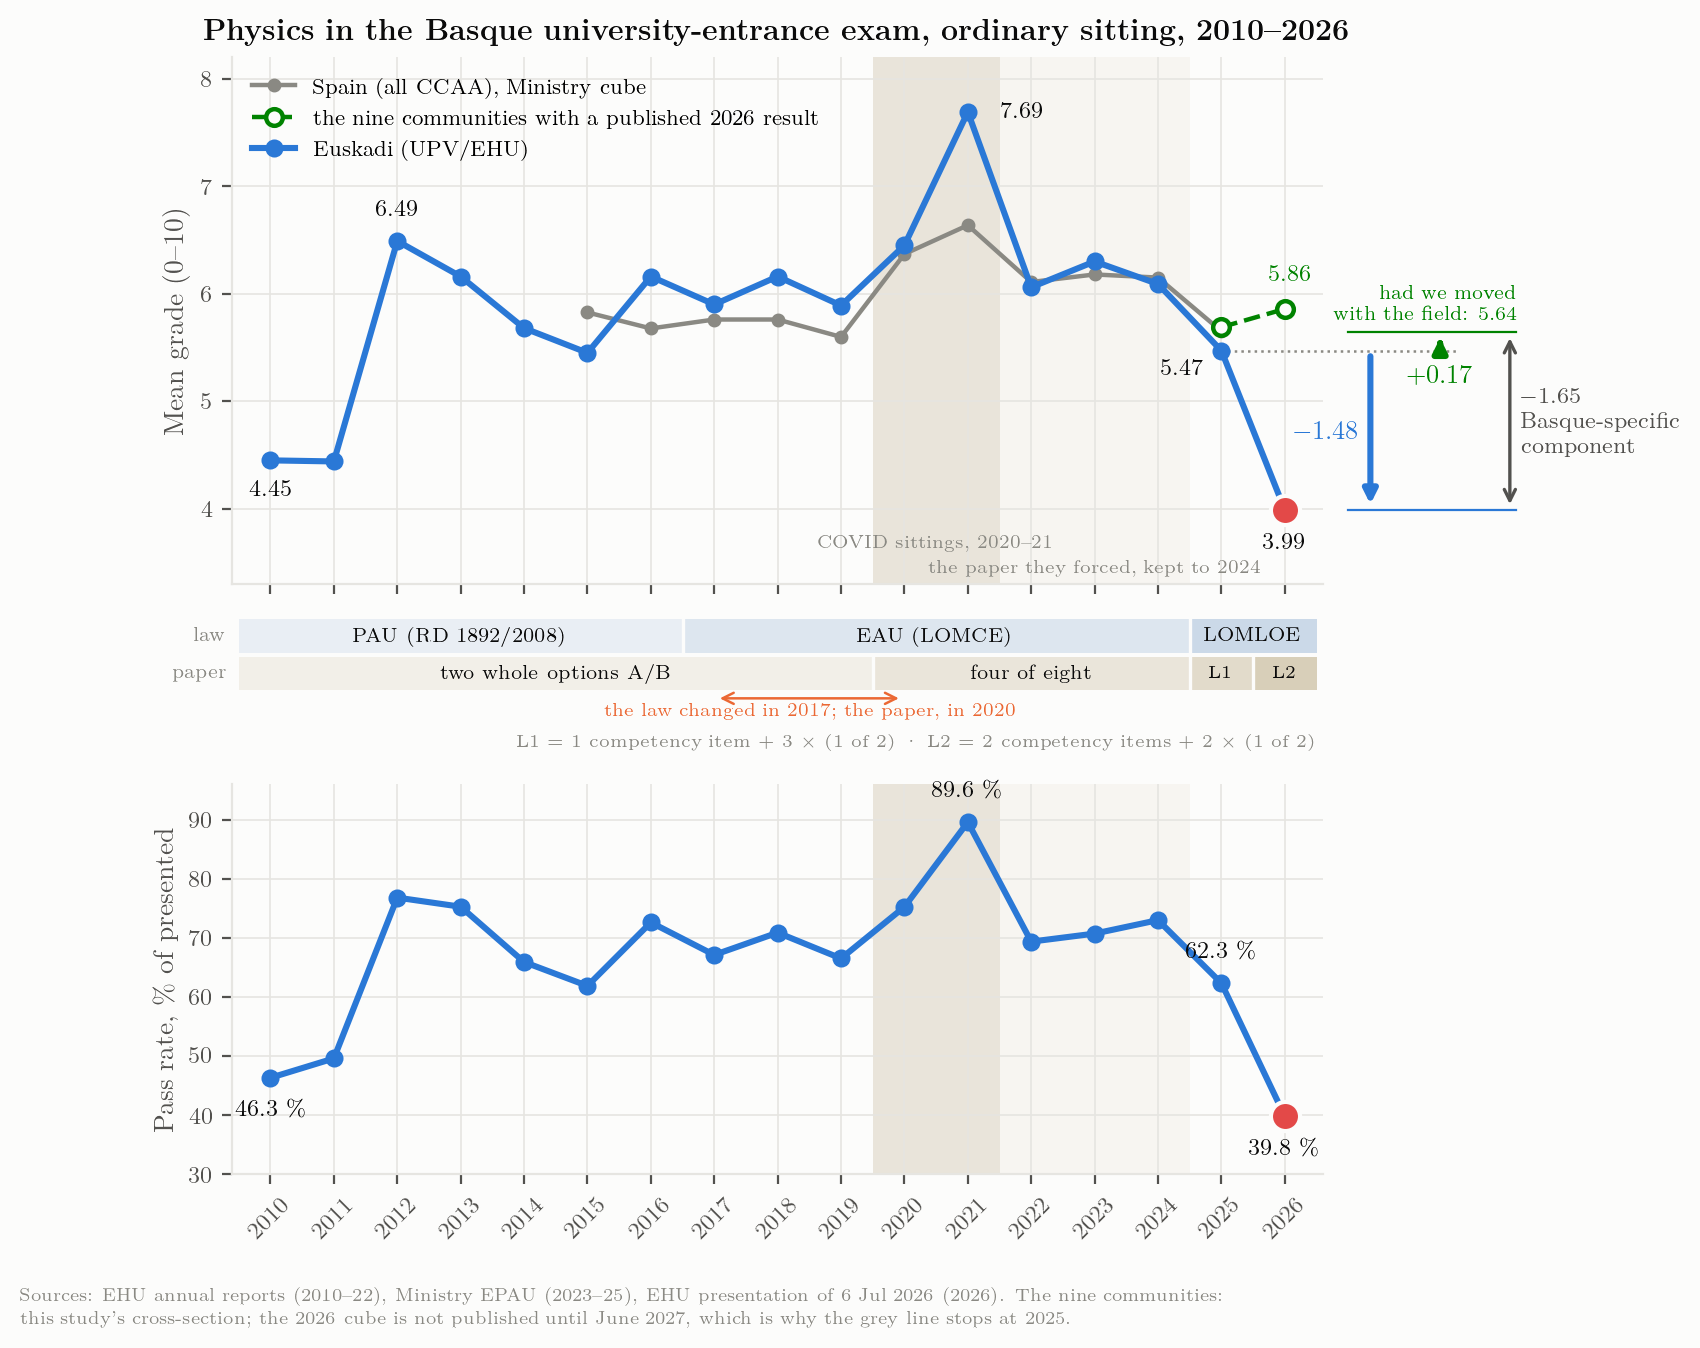
\includegraphics[keepaspectratio]{../plots/fig01_euskadi_series.png}}

}

\caption{\label{fig-b-series}Física in the Basque university-entrance
exam, ordinary sitting, 2010--2026. \textbf{The ribbon carries two
separate facts on the same axis}: the \emph{law} under which the exam
was set, and the \emph{paper model} actually used. They do not coincide
--- LOMCE governed from 2017 but the paper did not change until 2020,
and it changed then for COVID and not for the law --- which is why they
are two rows and not one band; the marked interval under them spans
those two years. \texttt{L1} and \texttt{L2} are the two LOMLOE papers,
keyed beneath. \textbf{COVID is two sittings and one model}: the darker
tint is 2020 and 2021, both set under the relief measures --- 2021 is
the highest mean in the series, 7.69 --- and the lighter one the
four-of-eight paper they forced, which was then kept through 2024.
\textbf{The grey line is the Ministry cube} for all seventeen
communities and stops at 2025, because the 2026 cube is not published
until June 2027. \textbf{The green marks} are this study's own
cross-section of the nine communities that have published a 2026 result
--- a different population, and drawn detached for that reason.
\textbf{The two arrows on the right are changes, not levels}, and both
leave the same point, Euskadi's own 2025 mean of 5.47. The \textbf{blue}
arrow is Euskadi's own change to 3.99, \(-1.48\). The \textbf{green}
arrow is the change of the nine-community field, \(+0.17\), drawn from
that same origin so that its head at 5.64 reads as \emph{where Física
would have ended had it moved with the field}. The bracket between the
two heads is therefore the Basque-specific component, \(-1.65\),
exactly. The distance between the two 2026 \textbf{levels} is 1.87 and
is \emph{not} that component, because the two series did not start level
in 2025 (5.47 against 5.69). The field is the mean of the nine
\textbf{including} Euskadi, which is the conservative reading; against
the eight others alone the component would be \(-1.86\). The three
values are the \texttt{total}, \texttt{common} and
\texttt{basque\_specific} terms of
\texttt{data/analysis/decomposition.json}, computed by
\texttt{scripts/21\_decay\_decomposition.py}. The Basque series is
spliced from the EHU annual reports (2010--2022, all phases), the
Ministry cube (2023--2025) and the EHU deck (2026); the three agree to
±0.02 where they overlap.}

\end{figure}%

Three facts about the level {[}Ch. 2{]}:

\begin{itemize}
\tightlist
\item
  \textbf{3.99 is the lowest value of the whole series}, below the
  2010--11 start of the two-phase PAU (4.45, 4.44). From 2012 to 2024
  the exam produced means between 5.45 and 6.49 in every year but the
  COVID peak of 2021; a flat trend fitted to those twelve years leaves
  2025 at \(-0.69\) and 2026 at \(-2.18\), which is seven residual
  standard deviations.
\item
  \textbf{It is the second consecutive fall}:
  \(6.09 \to 5.47 \to 3.99\). Against Euskadi's own pre-COVID norm the
  2026 sitting is \(-1.93\) on the Ministry's specific-phase series,
  \(-1.91\) pooled and \(-1.92\) on EHU's own published series --- a
  third larger than the \(-1.48\) in circulation, because 2025 was
  already 0.45 below that norm. (Three conventions, three numbers within
  two hundredths; this briefing uses the pooled one wherever communities
  are compared.)
\item
  \textbf{A single-year change of \(-1.48\) is rare but not
  unprecedented.} Across the 170 year-to-year changes in the Ministry
  panel (17 communities × 10 transitions, SD 0.74) exactly seven were as
  negative: Extremadura 2024 (\(-2.10\)), Cantabria 2017 (\(-1.94\)),
  Canarias 2019 (\(-1.76\)), Baleares 2025 (\(-1.65\)), Euskadi 2022
  (\(-1.62\), the post-COVID normalisation), Asturias 2025 (\(-1.55\))
  and Cantabria 2025 (\(-1.51\)). What is exceptional is the
  \emph{level}, and the two falls in a row.
\end{itemize}

\section{What happened elsewhere in
Spain}\label{what-happened-elsewhere-in-spain}

In 2025, the first year of the LOMLOE competency exam, the Física mean
fell in \textbf{14 of 17} communities by \(-0.81\) on average; Euskadi's
\(-0.62\) was \emph{milder} than the national move. In 2026, nine
communities have a published result:

\begin{longtable}[]{@{}
  >{\raggedright\arraybackslash}p{(\linewidth - 8\tabcolsep) * \real{0.2200}}
  >{\raggedleft\arraybackslash}p{(\linewidth - 8\tabcolsep) * \real{0.1000}}
  >{\raggedleft\arraybackslash}p{(\linewidth - 8\tabcolsep) * \real{0.1000}}
  >{\raggedleft\arraybackslash}p{(\linewidth - 8\tabcolsep) * \real{0.1000}}
  >{\raggedright\arraybackslash}p{(\linewidth - 8\tabcolsep) * \real{0.4800}}@{}}
\caption{The nine 2026 results found. Official unless marked press; the
2025 comparator is the Ministry's except for Cataluña, which is compared
with itself on the aptes basis. The cross-section is unweighted: Madrid
and Extremadura count equally {[}Ch.
3{]}.}\label{tbl-b-regions}\tabularnewline
\toprule\noalign{}
\begin{minipage}[b]{\linewidth}\raggedright
Community
\end{minipage} & \begin{minipage}[b]{\linewidth}\raggedleft
2025
\end{minipage} & \begin{minipage}[b]{\linewidth}\raggedleft
2026
\end{minipage} & \begin{minipage}[b]{\linewidth}\raggedleft
Δ
\end{minipage} & \begin{minipage}[b]{\linewidth}\raggedright
Basis
\end{minipage} \\
\midrule\noalign{}
\endfirsthead
\toprule\noalign{}
\begin{minipage}[b]{\linewidth}\raggedright
Community
\end{minipage} & \begin{minipage}[b]{\linewidth}\raggedleft
2025
\end{minipage} & \begin{minipage}[b]{\linewidth}\raggedleft
2026
\end{minipage} & \begin{minipage}[b]{\linewidth}\raggedleft
Δ
\end{minipage} & \begin{minipage}[b]{\linewidth}\raggedright
Basis
\end{minipage} \\
\midrule\noalign{}
\endhead
\bottomrule\noalign{}
\endlastfoot
Asturias & 5.49 & 6.62 & \(+1.13\) & presented, 76.9 \% pass ---
\textbf{press} (Uniovi release, not archived) \\
Madrid & 5.65 & 6.70 & \(+1.05\) & chart labels, one decimal \\
Castilla-La Mancha & 5.86 & 6.80 & \(+0.94\) & presented, n = 1 781 \\
Cataluña & 6.04 & 6.84 & \(+0.80\) & eligible students (``aptes'') both
years, n = 8 021 \\
Comunitat Valenciana & 5.89 & 6.40 & \(+0.51\) & presented, n = 5 259 \\
Andalucía & 5.69 & 5.86 & \(+0.17\) & presented \\
Extremadura & 6.09 & 5.27 & \(-0.82\) & \textbf{press} \\
Canarias (ULL + ULPGC) & 5.08 & 4.25 & \(-0.83\) & presented, n = 1
395 \\
País Vasco & 5.47 & 3.99 & \(-1.48\) & presented, n = 2 066 \\
\end{longtable}

\begin{figure}[htbp]

\centering{

\pandocbounded{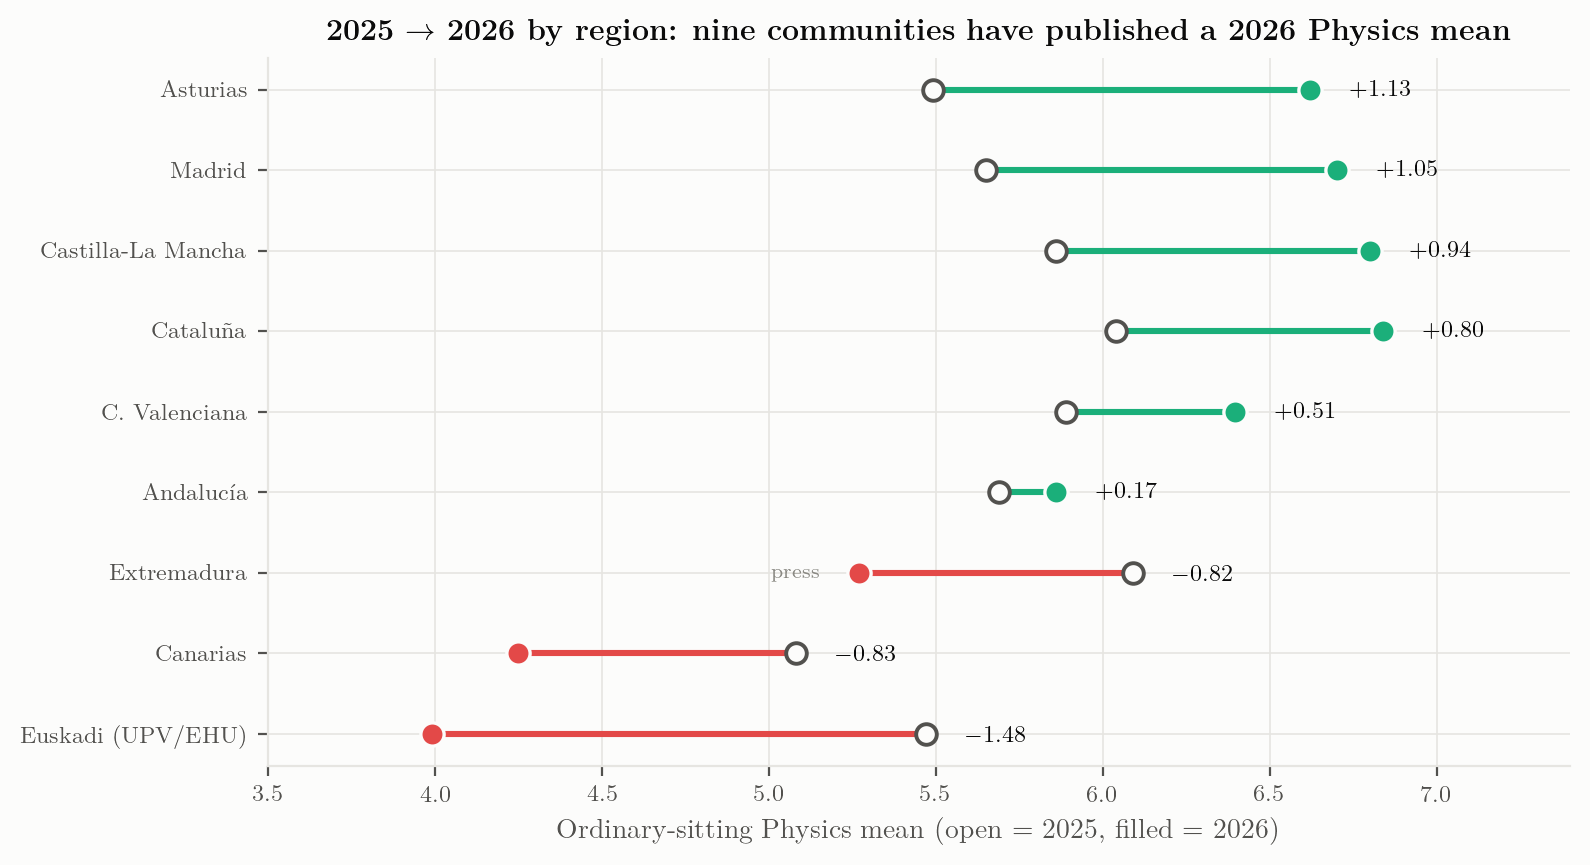
\includegraphics[keepaspectratio]{../plots/fig03_regions_2026_vs_2025.png}}

}

\caption{\label{fig-b-regions}2025 → 2026 by community: open circle
2025, filled 2026; red fell, green rose. Cataluña is on its aptes basis
in both years, Madrid's values are chart labels rounded to one decimal,
Extremadura's 2026 value is press-reported.}

\end{figure}%

Six communities rose under the same national model in the same year;
three fell. A national cause cannot produce opposite signs in the same
year, so \textbf{the competency model can at most describe 2025; it does
not explain 2026}. The eight remaining communities have published
nothing; the Ministry's 2026 cube is due in June 2027.

There is a second reason not to read 2025 as a national collapse.
Measured against each community's own 2015--2019 norm,
\textbf{2020--2024 was a plateau, not a decline}: the nine communities
sat \(+0.50\) to \(+1.05\) above their pre-COVID norm in every one of
those years and returned to it in 2025 in a single step. The plateau is
in every subject in the Ministry cube, and in 2025 every science subject
came back to within about a fifth of a point of its norm while the
humanities kept part of the lift. So the reform arrived in the same year
as the end of a subject-general regime, and nothing in the PAU series
separates the two. Against those norms the nine communities finish 2026
at \(+0.02\) on average --- but that average hides 2.9 points of spread,
from Madrid at \(+1.02\) to País Vasco at \(-1.91\).

\section{What the fall is made of}\label{what-the-fall-is-made-of}

This is the part of the briefing that bears on 2027, and it is new: it
asks not how large the fall was but how many distinct things happened
and which of them can be told apart.

\begin{figure}[htbp]

\centering{

\pandocbounded{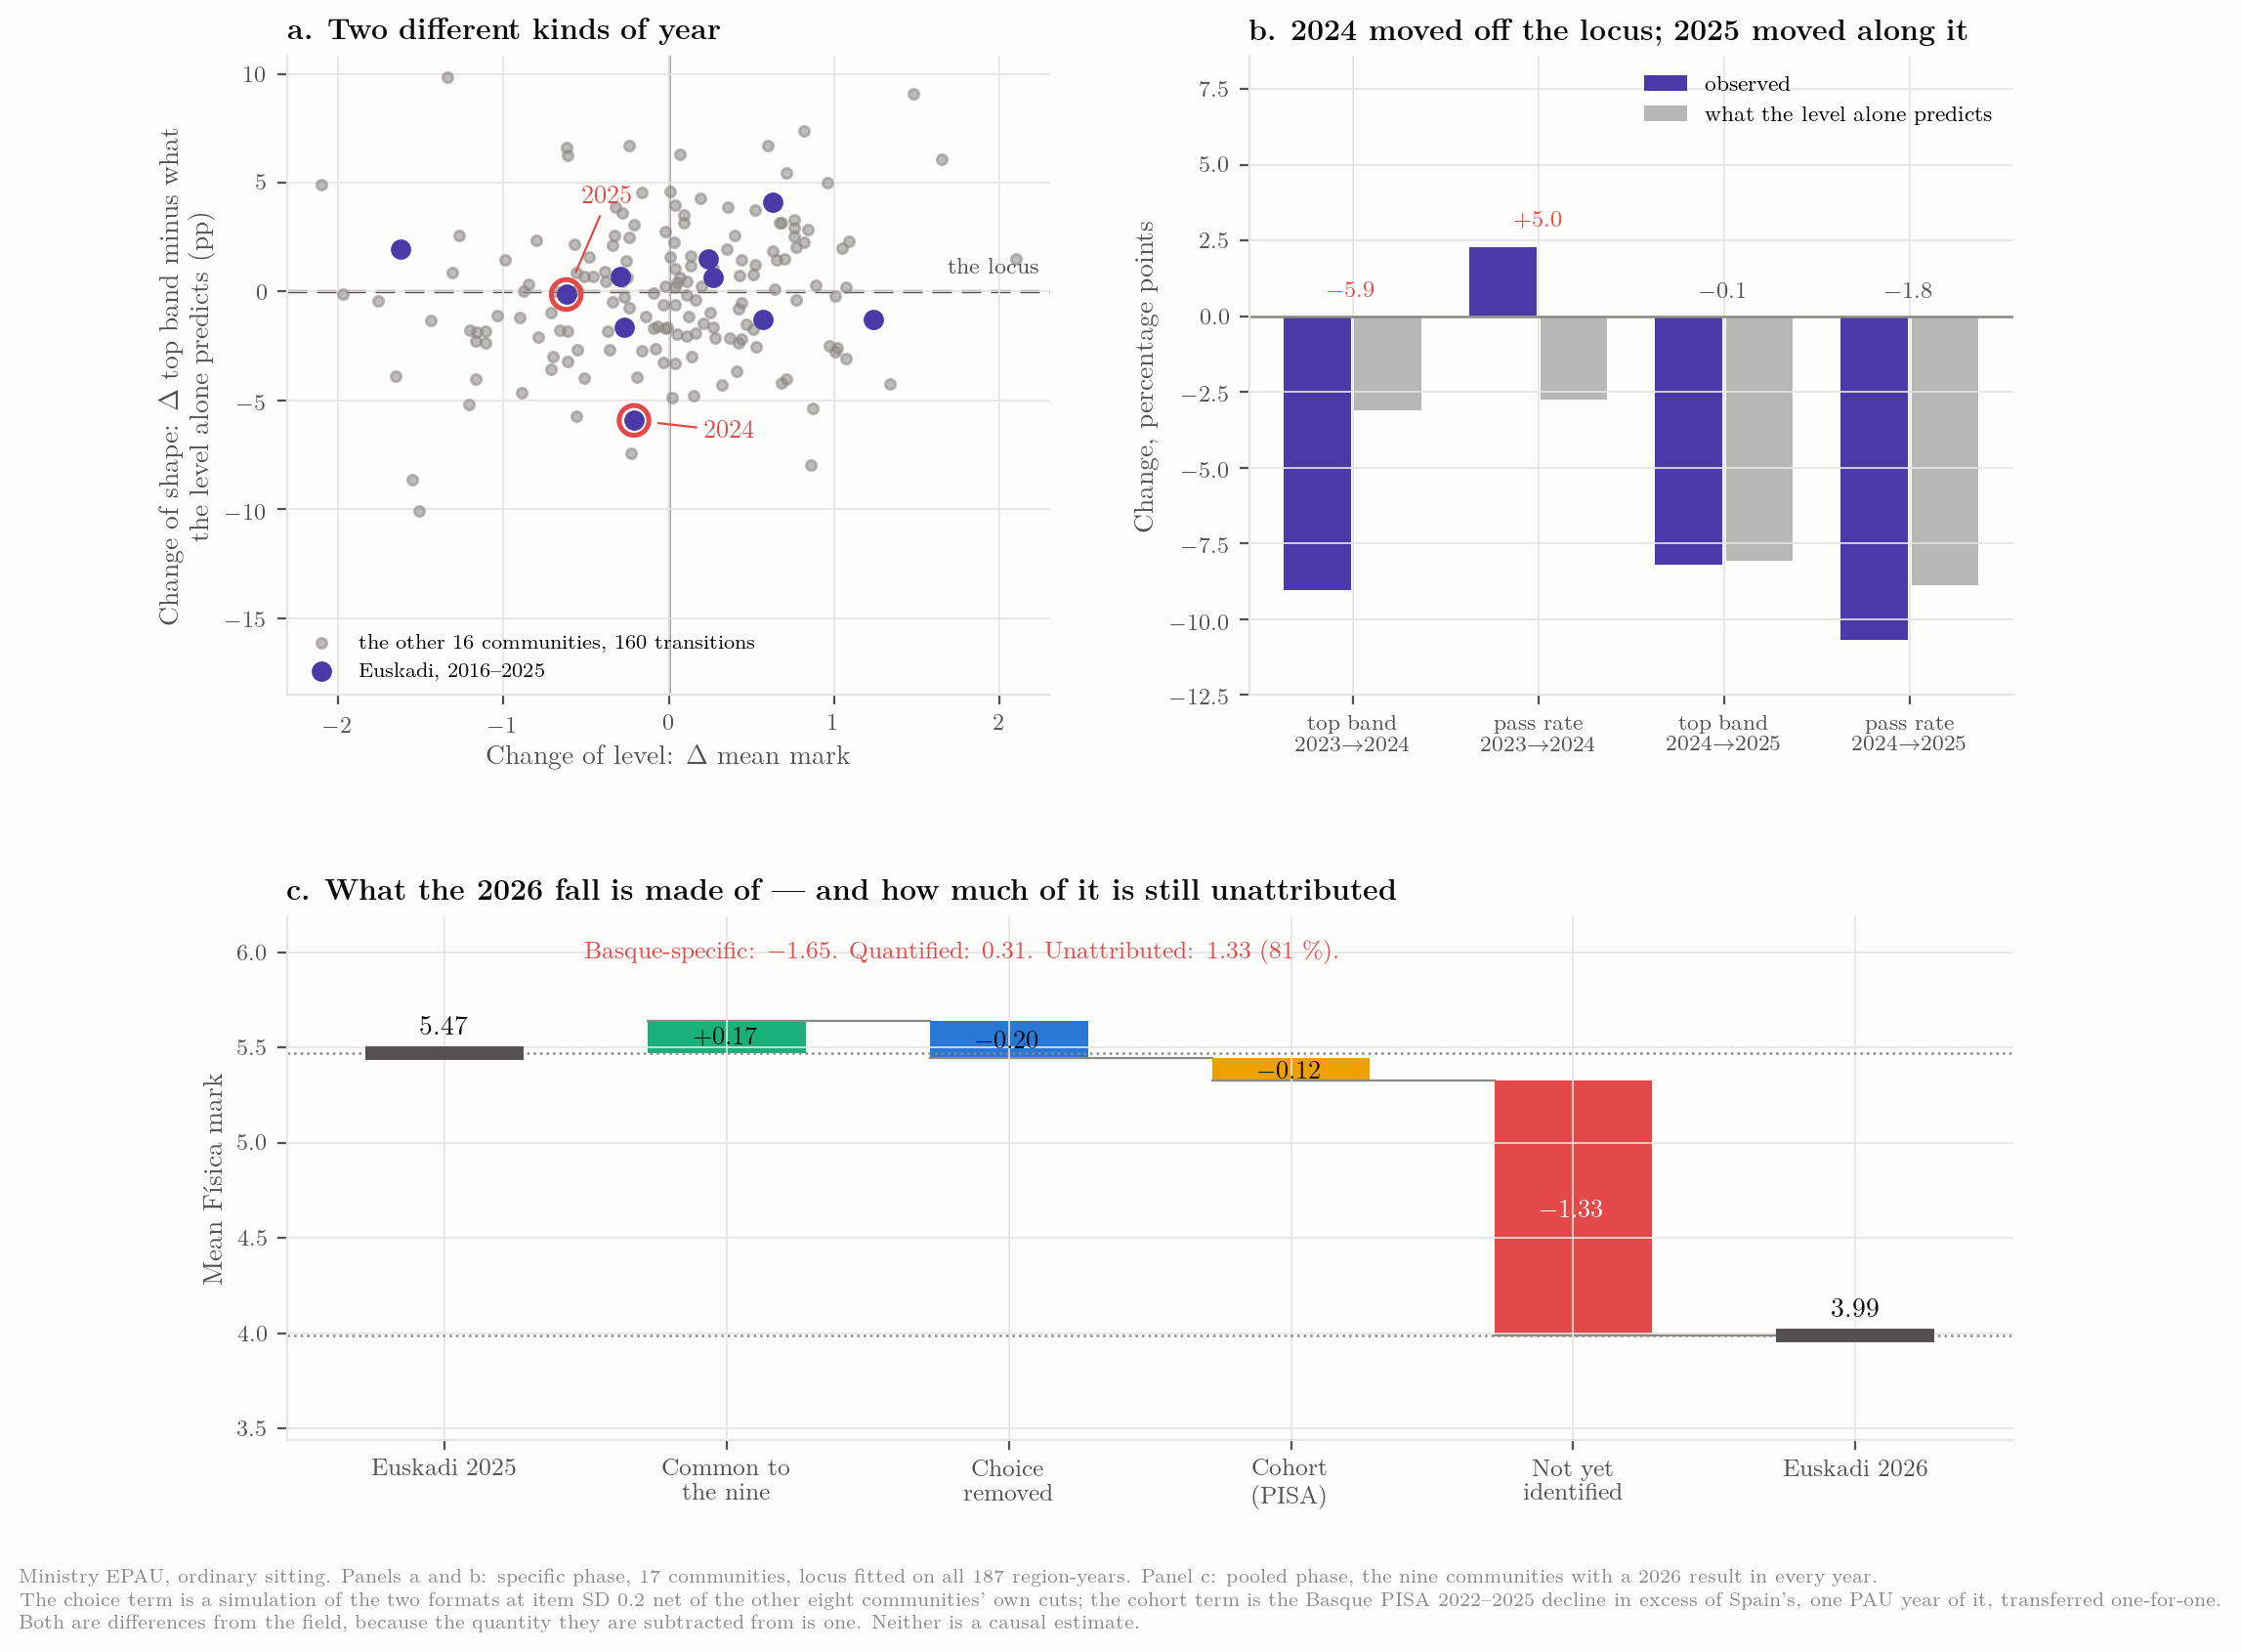
\includegraphics[keepaspectratio]{../plots/fig25_decomposition.png}}

}

\caption{\label{fig-b-decomp}\textbf{a} --- every year-to-year
transition in the national panel, placed by how much the mean moved and
by how far the top band moved away from what that change of mean alone
predicts. Euskadi's are violet; 2024 and 2025 are ringed. \textbf{b} ---
those two Basque years, observed against the prediction, for both
published band quantities. \textbf{c} --- the 2025 → 2026 fall split
into the part common to the nine reporting communities, the two
Basque-specific parts that can be quantified, and the part that cannot.}

\end{figure}%

\subsection{Three events, not one}\label{three-events-not-one}

A distribution can move in two ways: \textbf{location} (everything
slides together, and the pass rate and the top band move exactly as the
mean implies) or \textbf{shape} (they do not). The published aggregates
can tell them apart, and the three recent Basque years are not the same
kind of event.

\begin{longtable}[]{@{}
  >{\raggedright\arraybackslash}p{(\linewidth - 16\tabcolsep) * \real{0.1400}}
  >{\raggedleft\arraybackslash}p{(\linewidth - 16\tabcolsep) * \real{0.1000}}
  >{\raggedleft\arraybackslash}p{(\linewidth - 16\tabcolsep) * \real{0.1100}}
  >{\raggedleft\arraybackslash}p{(\linewidth - 16\tabcolsep) * \real{0.1200}}
  >{\raggedleft\arraybackslash}p{(\linewidth - 16\tabcolsep) * \real{0.1000}}
  >{\raggedleft\arraybackslash}p{(\linewidth - 16\tabcolsep) * \real{0.1000}}
  >{\raggedleft\arraybackslash}p{(\linewidth - 16\tabcolsep) * \real{0.1000}}
  >{\raggedleft\arraybackslash}p{(\linewidth - 16\tabcolsep) * \real{0.1200}}
  >{\raggedright\arraybackslash}p{(\linewidth - 16\tabcolsep) * \real{0.1200}}@{}}
\caption{The Basque steps against the locus fitted on all 187
region-years {[}Ch. 6{]}.}\label{tbl-b-steps}\tabularnewline
\toprule\noalign{}
\begin{minipage}[b]{\linewidth}\raggedright
Year
\end{minipage} & \begin{minipage}[b]{\linewidth}\raggedleft
Δ mean
\end{minipage} & \begin{minipage}[b]{\linewidth}\raggedleft
Δ top band
\end{minipage} & \begin{minipage}[b]{\linewidth}\raggedleft
what the level predicts
\end{minipage} & \begin{minipage}[b]{\linewidth}\raggedleft
excess
\end{minipage} & \begin{minipage}[b]{\linewidth}\raggedleft
Δ pass \%
\end{minipage} & \begin{minipage}[b]{\linewidth}\raggedleft
predicted
\end{minipage} & \begin{minipage}[b]{\linewidth}\raggedleft
excess
\end{minipage} & \begin{minipage}[b]{\linewidth}\raggedright
Reads as
\end{minipage} \\
\midrule\noalign{}
\endfirsthead
\toprule\noalign{}
\begin{minipage}[b]{\linewidth}\raggedright
Year
\end{minipage} & \begin{minipage}[b]{\linewidth}\raggedleft
Δ mean
\end{minipage} & \begin{minipage}[b]{\linewidth}\raggedleft
Δ top band
\end{minipage} & \begin{minipage}[b]{\linewidth}\raggedleft
what the level predicts
\end{minipage} & \begin{minipage}[b]{\linewidth}\raggedleft
excess
\end{minipage} & \begin{minipage}[b]{\linewidth}\raggedleft
Δ pass \%
\end{minipage} & \begin{minipage}[b]{\linewidth}\raggedleft
predicted
\end{minipage} & \begin{minipage}[b]{\linewidth}\raggedleft
excess
\end{minipage} & \begin{minipage}[b]{\linewidth}\raggedright
Reads as
\end{minipage} \\
\midrule\noalign{}
\endhead
\bottomrule\noalign{}
\endlastfoot
2023 → 2024 & \(-0.21\) & \(-9.0\) & \(-3.1\) & \(\mathbf{-5.9}\) &
\(+2.3\) & \(-2.8\) & \(\mathbf{+5.0}\) & \textbf{shape} \\
2024 → 2025 & \(-0.62\) & \(-8.2\) & \(-8.1\) & \(-0.1\) & \(-10.7\) &
\(-8.9\) & \(-1.8\) & \textbf{location} \\
2025 → 2026 & \(-1.48\) & --- & --- & --- & --- & --- & --- & not
published \\
\end{longtable}

\textbf{2024 changed the shape and barely touched the level.} The mean
moved 0.21 in a series whose year-to-year standard deviation is 0.85 ---
nothing. But the top band fell nine points where the level predicts
three, and the pass rate \emph{rose} two where the level predicts a fall
of three. The distribution compressed: fewer at the top, more just over
the line. As a move of the conditional top-band residual it is the
\textbf{second-most-negative of the 170 transitions} in the national
panel, and the largest negative move outside the LOMLOE year (two
positive moves are larger in absolute size). It happened on the last
paper of the old format, with the old choice rule and the old theory
questions.

\textbf{2025 changed the level and not the shape}, and most of that
change was the country's, not Euskadi's.

\textbf{2026 cannot be classified}, because EHU has not published the
distribution. The two 2026 cohorts in Spain that do publish one --- the
two Canarian universities, at almost exactly the Basque level --- are
pure location shifts.

One consequence is worth spelling out, because it is easy to miss and it
governs how the rest of the dossier should be read. A distribution can
lose candidates from its top and gain them just above the pass line at
the same time, and the two movements cancel in the mean. That is
precisely what 2024 did: the 8--10 share fell 9.0 points while the pass
rate \emph{rose} 2.3, and what came out was a change in the mean of 0.21
--- a twentieth of what the two band moves were worth separately. So
every test in this dossier that works on the mean --- the reference
frames, the plateau comparison, Euskadi's rank among the communities ---
reports Euskadi at or near its own norm in 2024. Those tests are not
wrong. They are answering a question about the average candidate, and
the average candidate was where he had always been. The candidates who
disappeared were at the top, and a mean cannot see them leave when
others arrive from below. That is why this dossier reads the bands as
well as the mean, and it is why the first thing that moved in the Basque
exam moved in 2024, a year before the first LOMLOE paper.

\subsection{The mark budget}\label{the-mark-budget}

Of the 1.48 points lost between 2025 and 2026, how much is Euskadi's
own? Comparing with the nine communities that have a 2026 result --- the
same nine in every year, so the comparison population never changes:

\begin{longtable}[]{@{}
  >{\raggedright\arraybackslash}p{(\linewidth - 8\tabcolsep) * \real{0.1600}}
  >{\raggedleft\arraybackslash}p{(\linewidth - 8\tabcolsep) * \real{0.2200}}
  >{\raggedleft\arraybackslash}p{(\linewidth - 8\tabcolsep) * \real{0.2000}}
  >{\raggedleft\arraybackslash}p{(\linewidth - 8\tabcolsep) * \real{0.2200}}
  >{\raggedleft\arraybackslash}p{(\linewidth - 8\tabcolsep) * \real{0.2000}}@{}}
\caption{The Basque change split into the country's move and Euskadi's
own, pooled phase {[}Ch. 6{]}.}\label{tbl-b-budget}\tabularnewline
\toprule\noalign{}
\begin{minipage}[b]{\linewidth}\raggedright
Year
\end{minipage} & \begin{minipage}[b]{\linewidth}\raggedleft
Euskadi mean
\end{minipage} & \begin{minipage}[b]{\linewidth}\raggedleft
Δ total
\end{minipage} & \begin{minipage}[b]{\linewidth}\raggedleft
Common to the nine
\end{minipage} & \begin{minipage}[b]{\linewidth}\raggedleft
Basque-specific
\end{minipage} \\
\midrule\noalign{}
\endfirsthead
\toprule\noalign{}
\begin{minipage}[b]{\linewidth}\raggedright
Year
\end{minipage} & \begin{minipage}[b]{\linewidth}\raggedleft
Euskadi mean
\end{minipage} & \begin{minipage}[b]{\linewidth}\raggedleft
Δ total
\end{minipage} & \begin{minipage}[b]{\linewidth}\raggedleft
Common to the nine
\end{minipage} & \begin{minipage}[b]{\linewidth}\raggedleft
Basque-specific
\end{minipage} \\
\midrule\noalign{}
\endhead
\bottomrule\noalign{}
\endlastfoot
2024 & 6.09 & \(-0.21\) & \(-0.03\) & \(-0.18\) \\
2025 & 5.47 & \(-0.62\) & \(-0.65\) & \(+0.03\) \\
2026 & 3.99 & \(-1.48\) & \(+0.17\) & \(\mathbf{-1.65}\) \\
\end{longtable}

In 2025 Euskadi moved with the field to within three hundredths of a
point: \textbf{the whole of that year's fall was national}. In 2026 the
field rose \(+0.17\) and Euskadi fell \(-1.48\), so the Basque-specific
component is \textbf{\(-1.65\)}.

That is the number to explain --- not 1.48, which mixes a national
recovery into a Basque fall, and not 1.93, which is the same thing
measured from a different year.

\subsection{Which frame, and does it
matter}\label{which-frame-and-does-it-matter}

Why measure a Basque fall against a Spanish field at all, when the
question is what happened in Euskadi? Three frames give three numbers:

\begin{longtable}[]{@{}
  >{\raggedright\arraybackslash}p{(\linewidth - 4\tabcolsep) * \real{0.2800}}
  >{\raggedright\arraybackslash}p{(\linewidth - 4\tabcolsep) * \real{0.5000}}
  >{\raggedleft\arraybackslash}p{(\linewidth - 4\tabcolsep) * \real{0.2200}}@{}}
\caption{The same result, three frames {[}Ch.
6{]}.}\label{tbl-b-frames}\tabularnewline
\toprule\noalign{}
\begin{minipage}[b]{\linewidth}\raggedright
Frame
\end{minipage} & \begin{minipage}[b]{\linewidth}\raggedright
What it asks
\end{minipage} & \begin{minipage}[b]{\linewidth}\raggedleft
2026
\end{minipage} \\
\midrule\noalign{}
\endfirsthead
\toprule\noalign{}
\begin{minipage}[b]{\linewidth}\raggedright
Frame
\end{minipage} & \begin{minipage}[b]{\linewidth}\raggedright
What it asks
\end{minipage} & \begin{minipage}[b]{\linewidth}\raggedleft
2026
\end{minipage} \\
\midrule\noalign{}
\endhead
\bottomrule\noalign{}
\endlastfoot
Year on year & how far did the Basque mean fall from 2025? &
\(-1.48\) \\
Against Euskadi's own pre-COVID norm & how far is 2026 from where
Euskadi normally sits? & \(-1.91\) \\
Against the nine-community field & how much is Euskadi's own, once the
country's move is out? & \(-1.65\) \\
\end{longtable}

They span 0.43 of a mark. Nothing in this briefing turns on the choice,
and every design implication below is the same under all three.

What the field buys is not size but \textbf{separation}, for one purpose
no absolute number can serve: telling a year in which everyone fell from
a year in which only Euskadi did. Read absolutely, Euskadi lost 0.62
marks in 2025 and that looks like a Basque problem. Read against the
field, which lost 0.65 in the same sitting, there is nothing Basque in
2025 at all, and the whole of the anomaly is in 2026. Without the field
the two years look like one slide of 2.10 marks; with it, they are one
national event followed by one Basque event, and only the second is this
office's to answer.

What the field is \textbf{not} is a control group, and the arithmetic
should not be allowed to imply otherwise. These nine sat nine different
papers, marked to nine different criteria, by nine different sets of
correctors. Euskadi is the only community that moved all four reform
axes in the direction the orientations ask for (optionality 75 \% → 50
\%, competency marks 25 \% → 62.5 \%, substantive context \(+50\),
contextualised marks \(+75\)); Castilla-La Mancha is the only other that
both cut choice and raised competency content, and it cut contextualised
marks by 45 points while doing so; Cataluña moved the competency share
the other way; three communities moved on no axis but the contextualised
share; and Asturias, which rose \(+1.13\), sits outside the structural
optionality band altogether at 100 \% {[}Ch. 11{]}. Across the nine, the
further a paper moved toward the competency model the further its mean
fell (\(r = -0.70\), \(p = 0.035\)) --- but Euskadi is the extreme point
on both axes and dropping it leaves \(r = -0.40\), \(p = 0.33\), so that
is one community making the point rather than eight agreeing.

The practical consequence is a range. Against all eight other
communities the Basque-specific component is \(-1.65\); against the six
whose papers barely moved, \(-1.95\); against nothing at all, \(-1.48\).
It is somewhere in \([-1.95, -1.48]\), and it cannot be narrowed because
nobody has calibrated these nine papers against each other. That is data
request 9.

\subsection{Is the 1.65 Física's, or
Euskadi's?}\label{is-the-1.65-fuxedsicas-or-euskadis}

The budget is computed on Física alone, so it cannot distinguish two
situations that call for different responses: something that happened to
the \emph{Física paper}, or something that happened to \emph{Euskadi}
--- its cohort, its tribunals, its marking --- and landed on Física
along with everything else.

The subject results separate them without any modelling. EHU published
eight subjects; four comparator communities published three of the same
ones, giving a balanced five-by-three panel on which the Basque Física
change splits into four terms that sum exactly to \(-1.48\).

{

\begin{longtable}[]{@{}
  >{\raggedright\arraybackslash}p{(\linewidth - 10\tabcolsep) * \real{0.1304}}
  >{\raggedleft\arraybackslash}p{(\linewidth - 10\tabcolsep) * \real{0.1739}}
  >{\raggedleft\arraybackslash}p{(\linewidth - 10\tabcolsep) * \real{0.1739}}
  >{\raggedleft\arraybackslash}p{(\linewidth - 10\tabcolsep) * \real{0.1739}}
  >{\raggedleft\arraybackslash}p{(\linewidth - 10\tabcolsep) * \real{0.1739}}
  >{\raggedleft\arraybackslash}p{(\linewidth - 10\tabcolsep) * \real{0.1739}}@{}}

\caption{\label{tbl-b-subj}The balanced panel behind the split {[}Ch.
6{]}.}

\tabularnewline

\toprule\noalign{}
\begin{minipage}[b]{\linewidth}\raggedright
Community
\end{minipage} & \begin{minipage}[b]{\linewidth}\raggedleft
Física
\end{minipage} & \begin{minipage}[b]{\linewidth}\raggedleft
Matemáticas II
\end{minipage} & \begin{minipage}[b]{\linewidth}\raggedleft
Química
\end{minipage} & \begin{minipage}[b]{\linewidth}\raggedleft
Mean of the three
\end{minipage} & \begin{minipage}[b]{\linewidth}\raggedleft
Física − own mean
\end{minipage} \\
\midrule\noalign{}
\endhead
\bottomrule\noalign{}
\endlastfoot
País Vasco & -1.48 & -1.67 & -0.21 & -1.12 & -0.36 \\
Cataluña & +0.80 & -1.94 & -0.34 & -0.49 & +1.29 \\
Madrid & +1.10 & +0.50 & -0.30 & +0.43 & +0.67 \\
Andalucía & +0.17 & -0.59 & -0.22 & -0.21 & +0.38 \\
Asturias & +1.13 & +0.10 & +0.28 & +0.50 & +0.63 \\
\textbf{Field (four communities)} & +0.80 & -0.48 & -0.15 & +0.06 &
+0.74 \\

\end{longtable}

}

Change in the subject mean, 2025 to 2026, in marks out of ten. The last
two columns are the terms of the additive split: a community's mean over
the three subjects, and how far its Física sits from that mean.

\begin{longtable}[]{@{}
  >{\raggedright\arraybackslash}p{(\linewidth - 4\tabcolsep) * \real{0.2400}}
  >{\raggedleft\arraybackslash}p{(\linewidth - 4\tabcolsep) * \real{0.1200}}
  >{\raggedright\arraybackslash}p{(\linewidth - 4\tabcolsep) * \real{0.6400}}@{}}
\caption{The exact split of the \(-1.48\) {[}Ch.
6{]}.}\label{tbl-b-split}\tabularnewline
\toprule\noalign{}
\begin{minipage}[b]{\linewidth}\raggedright
Term
\end{minipage} & \begin{minipage}[b]{\linewidth}\raggedleft
Marks
\end{minipage} & \begin{minipage}[b]{\linewidth}\raggedright
What it is
\end{minipage} \\
\midrule\noalign{}
\endfirsthead
\toprule\noalign{}
\begin{minipage}[b]{\linewidth}\raggedright
Term
\end{minipage} & \begin{minipage}[b]{\linewidth}\raggedleft
Marks
\end{minipage} & \begin{minipage}[b]{\linewidth}\raggedright
What it is
\end{minipage} \\
\midrule\noalign{}
\endhead
\bottomrule\noalign{}
\endlastfoot
Field core & \(+0.06\) & what the three shared subjects did in the four
comparators \\
Field Física premium & \(+0.74\) & Física above its own community's mean
in all four; the mean of \(+0.38\) to \(+1.29\) \\
\textbf{Euskadi-common} & \(\mathbf{-1.18}\) & what moved all of
Euskadi's quantitative subjects together \\
\textbf{Física-specific} & \(\mathbf{-1.10}\) & what is left for the
Física paper \\
\end{longtable}

Add the two Euskadi terms and Euskadi's Física sits \textbf{2.28 marks
below what these four comparators' Física did} --- the four-community
analogue of the \(-1.65\), larger because these four are among the
communities that rose most, and no more a control than the nine are.
What the split adds is the proportion: \textbf{slightly more than half
of that gap, 1.18 of 2.28, is not Física's.} In the same sitting, at the
same university, under the same marking specification, Matemáticas II
lost 1.67 marks --- more than Física --- while Química (\(-0.21\)),
Biología (\(+0.15\)) and Lengua Castellana (\(+0.03\)) did not follow.

That changes what the 2027 Física paper can be expected to fix.
Rewriting it addresses the \(-1.10\). It does not touch the \(-1.18\),
which is invisible to anything decided inside one subject's
\emph{ponencia}, and which the Matemáticas II coordination is presumably
looking at from its own side without either group seeing the shared
term. \textbf{The first operational consequence of this briefing is
therefore that Física and Matemáticas II should be looked at together,
and that is a decision for this office rather than for either ponencia.}

One caution: the comparator set is four communities and three subjects
because that is all that was published by mid-September, and each of
those communities changed its own papers too. A symmetric analysis of
variance over all five leaves the Física-specific residual at \(-0.88\)
rather than \(-1.10\); the conclusion --- that the Euskadi-wide term is
of the same order as the Física-specific one --- holds either way.

\subsection{What can be subtracted, and what
cannot}\label{what-can-be-subtracted-and-what-cannot}

\begin{longtable}[]{@{}
  >{\raggedright\arraybackslash}p{(\linewidth - 8\tabcolsep) * \real{0.2700}}
  >{\raggedleft\arraybackslash}p{(\linewidth - 8\tabcolsep) * \real{0.1000}}
  >{\raggedright\arraybackslash}p{(\linewidth - 8\tabcolsep) * \real{0.1400}}
  >{\raggedright\arraybackslash}p{(\linewidth - 8\tabcolsep) * \real{0.2200}}
  >{\raggedright\arraybackslash}p{(\linewidth - 8\tabcolsep) * \real{0.2700}}@{}}
\caption{Components of the Basque-specific 2026 change {[}Ch.
6{]}.}\label{tbl-b-components}\tabularnewline
\toprule\noalign{}
\begin{minipage}[b]{\linewidth}\raggedright
Component
\end{minipage} & \begin{minipage}[b]{\linewidth}\raggedleft
Marks
\end{minipage} & \begin{minipage}[b]{\linewidth}\raggedright
Range
\end{minipage} & \begin{minipage}[b]{\linewidth}\raggedright
Status
\end{minipage} & \begin{minipage}[b]{\linewidth}\raggedright
What would identify it
\end{minipage} \\
\midrule\noalign{}
\endfirsthead
\toprule\noalign{}
\begin{minipage}[b]{\linewidth}\raggedright
Component
\end{minipage} & \begin{minipage}[b]{\linewidth}\raggedleft
Marks
\end{minipage} & \begin{minipage}[b]{\linewidth}\raggedright
Range
\end{minipage} & \begin{minipage}[b]{\linewidth}\raggedright
Status
\end{minipage} & \begin{minipage}[b]{\linewidth}\raggedright
What would identify it
\end{minipage} \\
\midrule\noalign{}
\endhead
\bottomrule\noalign{}
\endlastfoot
Common to the country & \(+0.17\) & --- & observed & already
separated \\
Choice removed, net of the field's own cuts & \(-0.20\) & \(-0.10\) to
\(-0.27\) & quantified (modelled) & option take-up and per-option
means \\
Cohort: Basque PISA decline in excess of Spain's & \(-0.12\) &
\(\pm 0.11\) (sampling error only) & quantified (modelled) & nothing
inside the PAU; it is an outside measure \\
Paper content and reading load & --- & --- & \textbf{not identified}
(the two are one signal, \(r = +0.79\)); the \emph{cause} of the length
is now measured, and it is the itemisation, not the competency items &
sub-task marks \\
Marking severity (penalties, voided sections) & --- & bounded: \(0.65\)
to \(0.96\) of the Física-specific \(-1.10\) & \textbf{sufficient, not
identified} & the penalty ledger crossed with each script's mark, and
the 2026 band table \\
Tribunal severity and spread & --- & --- & \textbf{not identified} &
Física by tribunal \\
Newly examined topics & --- & --- & \textbf{not identified} (bounded:
optional in June) & option take-up \\
Who sat the exam & --- & --- & \textbf{not identified} (bounded small) &
enrolment and the 2025-26 school marks \\
\end{longtable}

Two rows changed again in the seventh round, and one of them changed for
a reason that is not about marking at all. The \textbf{reading-load} row
is unchanged in what it claims --- the paper really is 39 per cent
longer to read, and length really does track the fall across the nine
communities --- but its \emph{cause} is no longer what this briefing
said. Splitting both papers' statements into narrative, demand text and
printed prices shows the contextual narrative at 71 words a printed
statement in 2025 and \textbf{70 in 2026}, while the demand text more
than doubled from 88 to 181 and the printed prices went from nothing to
17. The 2026 criteria itemise each apartado into sub-items of 0.25, and
a paper marked that way must print each quantum's demand and each
quantum's price. The length is the price of that decision
(\href{16-paradigm.qmd}{Ch. 16}). It matters here because the two causes
are differently actionable: the competency requirement is imposed, the
itemisation is local. The \textbf{marking} row tightens: only 14 to 19
of a script's 27 to 32 sub-items can attract a unit, prefix or rounding
error, so the fitted intensity restated in countable currency is 0.67
penalties on every numerical answer of every script; and the linguistic
channel, which this briefing twice called an unmodelled understatement,
is capped by the criteria at 1.00 and fitted at 0.04.

The marking row changed status in the fifth and sixth rounds and is
worth reading in full rather than from the table. What changed in 2026
was not markers becoming harsher on the same scale but a change of
\textbf{regime}: a defect that until 2025 cost the part of the sub-task
depending on it now costs that part \emph{and} \(-0.10\), uncapped, and
a grave error voids the whole apartado. Put the published 2025
distribution through that regime and the four published 2026 figures
come out together, on about twelve deductions per script
(\href{06-interpretation.qmd\#penalty-regime}{Ch. 6}). But that model
gives every candidate the same twelve, and when the penalties are
allowed to fall unevenly --- which is what anybody would expect --- the
regime is worth \textbf{less}, because a deduction removes a full
\(0.10\) only where \(0.10\) is left and the zero floor absorbs the rest
of any penalty aimed at weak work. Flat and equal is therefore the
\emph{most expensive} way to spend a fixed number of penalties, over
every reading in which the weaker candidates collect more than their
share. At twelve deductions the regime carries \(0.96\) marks read flat
and \(0.89\) to \(0.65\) read as a distribution: 87 \% down to 59 \% of
the Física-specific \(-1.10\)
(\href{06-interpretation.qmd\#penalty-shape}{Ch. 6}). \textbf{So this
row is a ceiling and a floor rather than an estimate}, and the
difference between them --- a fifth to nearly half a mark --- stays with
the rows above and below it. One unpublished table, the 2026 grade
bands, would close the interval: refitted to everything that \emph{is}
published, the readings differ on the share at nine or above from 0.3 \%
to 6.1 \%.

Two components can be quantified, and both have to be expressed as
differences \emph{from the field}, because the quantity they are
subtracted from is one. \textbf{Choice}: removing the option from two of
the four exercises is worth \(-0.26\) by simulating both Basque formats
on the same population and items; the other eight communities cut
optionality by 6.25 points on average, and whatever that cost is already
inside the \(+0.17\), so the part that belongs here is about
\textbf{\(-0.20\)}. \textbf{Cohort}: the Basque PISA decline in excess
of Spain's --- 13.6 of the 21.0 points --- is worth about
\textbf{\(-0.12\)} for one PAU year. Together \textbf{\(-0.31\)}, under
a fifth of the Basque-specific fall. Both are modelled magnitudes under
stated assumptions, not measurements: their quoted ranges are
sensitivities to one assumption each, and the cohort's \(\pm 0.11\)
covers PISA's sampling error and nothing else.

The other \textbf{\(-1.33\) --- four fifths --- is not attributed to
anything}, and the reason is structural rather than a gap in the work:
paper content, reading load, marking severity and syllabus exposure all
leave the same trace in a mean. Length and competency content are one
signal measured twice (\(r = +0.79\) across eight communities), and the
cross-community relation between length and grade change, taken
literally, would assign 2.3 marks to the Basque paper's 45 \%
lengthening --- more than the entire Basque-specific fall, which is
itself the reason not to take it literally.

\textbf{Four fifths of what happened is therefore a bundle, not a
mystery.} It has four named candidates, each with a different remedy,
and one dataset --- marks at the level of the sub-task --- would go a
long way towards separating them, though not perfectly: a section voided
by a grave error and a sub-task nobody could start both appear as a zero
on the same sub-task.

\subsection{Marking severity: the timing fits, and one version of it
survives}\label{marking-severity-the-timing-fits-and-one-version-of-it-survives}

2026 was the second year in which the linguistic component --- 0.2 of a
point for grammar, spelling and presentation --- and the seven
minor-error deductions of the marking specification were in force, and
the first in which correctors had already applied them once. The seven
are \(-0.10\) each and are written for numerical work: units, a vector
arrow missing from a vector, a vector arrow on a scalar, intermediate
rounding beyond 5 \%, a wrong SI prefix, a factor of ten, a
transcription error.

The hypothesis that a rule applied cautiously in year one is applied in
full in year two predicts little in 2025 and a step in 2026.
\textbf{That is exactly the shape of the mark budget}: the
Basque-specific component is \(+0.03\) in 2025 and \(-1.65\) in 2026.
The timing fits, and that should be on the record.

The eight-subject table then separates two versions of it, because they
predict different things.

{

\begin{longtable}[]{@{}
  >{\raggedright\arraybackslash}p{(\linewidth - 8\tabcolsep) * \real{0.1875}}
  >{\raggedleft\arraybackslash}p{(\linewidth - 8\tabcolsep) * \real{0.2500}}
  >{\raggedright\arraybackslash}p{(\linewidth - 8\tabcolsep) * \real{0.1875}}
  >{\centering\arraybackslash}p{(\linewidth - 8\tabcolsep) * \real{0.1875}}
  >{\centering\arraybackslash}p{(\linewidth - 8\tabcolsep) * \real{0.1875}}@{}}

\caption{\label{tbl-b-severity}The 2026 Basque subject changes grouped
by which marking rules can reach them {[}Ch. 6{]}.}

\tabularnewline

\toprule\noalign{}
\begin{minipage}[b]{\linewidth}\raggedright
Basque subject
\end{minipage} & \begin{minipage}[b]{\linewidth}\raggedleft
Change 2025→2026
\end{minipage} & \begin{minipage}[b]{\linewidth}\raggedright
Family
\end{minipage} & \begin{minipage}[b]{\linewidth}\centering
Reached by the 0.2 linguistic component
\end{minipage} & \begin{minipage}[b]{\linewidth}\centering
Reached by the seven minor-error rules
\end{minipage} \\
\midrule\noalign{}
\endhead
\bottomrule\noalign{}
\endlastfoot
Física & -1.48 & quantitative & yes & yes \\
Matemáticas II & -1.67 & quantitative & yes & yes \\
Química & -0.21 & quantitative & yes & yes \\
Historia de España & -0.83 & verbal / other & yes & no \\
Euskara II & -0.48 & verbal / other & yes & no \\
Hª Filosofía & -0.29 & verbal / other & yes & no \\
Biología & +0.15 & verbal / other & yes & no \\
Lengua Castellana & +0.03 & verbal / other & yes & no \\
\textbf{Quantitative mean} & \textbf{-1.12} & & & \\
\textbf{Verbal mean} & \textbf{-0.28} & & & \\
\textbf{Gap} & \textbf{-0.84} & & & \\

\end{longtable}

}

Both families are examined in the same sitting at the same university,
under the same marking specification and in the same second year of it
--- but by each subject's own correctors and on each subject's own
candidates, so this is not a within-person comparison. A marking change
written into the shared specification and applied across the board would
move both columns together; the gap is what such a change cannot
produce.

A \textbf{general} severity effect --- spelling, presentation, ``this
year we apply the criteria in full'' --- reaches every subject that asks
a candidate to write, which all eight of these do, and should move all
eight together. They did not: the spread is 1.82 marks, and of the three
subjects where written language is most exposed two rose (Lengua
Castellana \(+0.03\), Biología \(+0.15\)) while Euskara II fell
\(-0.48\). Whatever is common to all eight is at most the verbal mean of
\(-0.28\) --- on the condition that the 2026 verbal papers were no
easier than their predecessors, which is not known, since part of that
\(-0.28\) is the cohort and part each subject's own paper. \textbf{On
that condition a general severity effect accounts for at most a fifth of
Física's 1.48, and probably much less.}

A \textbf{quantitative-specific} severity effect is a different
proposition, and the pattern fits it: the deductions can only reach
Física, Química and Matemáticas II, and those three fell 0.84 marks
further than the other five. The fit is not strong evidence --- Química
fell only 0.21, so the effect would not be uniform over the subjects it
can reach, and Física and Matemáticas II share long symbolic derivations
and a 2026 format change as well as the deductions. Eight subjects in
one year is a pattern with a prediction attached, not a test.

\textbf{The test is cheap and the data already exist.} The linguistic
component and the seven deductions are recorded separately when applied.
A tally --- how many scripts lost the 0.2, how many \(-0.10\) penalties
per script and of which type, in Física, Matemáticas II, Lengua
Castellana and Euskara II, in 2025 and in 2026 --- turns the hypothesis
into two cross-tabulations. It collects nothing new and can be answered
from inside the university. It is \textbf{data request 3}, and it is the
only decisive item on that list obtainable in days rather than months.

One design consequence does not wait for the answer. The 2026 Basque
paper raised the competency-coded share of its expected marks from 25 \%
to 62.5 \%, the largest such move among the nine. Competency items ask
for a calculation \emph{and} an argument, so they are exposed to the
linguistic component and the numerical deductions at once, where a bare
calculation is exposed only to the second. If the deductions bite harder
on that compound surface, the format change and the second year of full
application are not two hypotheses but one --- and nothing published can
separate them, because both happened in Euskadi in June 2026 and in no
other community.

\section{The shape of the collapse}\label{the-shape-of-the-collapse}

Euskadi publishes four summary numbers; the two Canarian universities
publish full histograms and are the closest empirical picture of the
same event {[}Ch. 4{]}.

\begin{longtable}[]{@{}
  >{\raggedright\arraybackslash}p{(\linewidth - 12\tabcolsep) * \real{0.1111}}
  >{\raggedleft\arraybackslash}p{(\linewidth - 12\tabcolsep) * \real{0.1481}}
  >{\raggedleft\arraybackslash}p{(\linewidth - 12\tabcolsep) * \real{0.1481}}
  >{\raggedleft\arraybackslash}p{(\linewidth - 12\tabcolsep) * \real{0.1481}}
  >{\raggedleft\arraybackslash}p{(\linewidth - 12\tabcolsep) * \real{0.1481}}
  >{\raggedleft\arraybackslash}p{(\linewidth - 12\tabcolsep) * \real{0.1481}}
  >{\raggedleft\arraybackslash}p{(\linewidth - 12\tabcolsep) * \real{0.1481}}@{}}
\caption{The Canarian histograms, from the ULL and ULPGC dashboards
(official).}\label{tbl-b-canarias}\tabularnewline
\toprule\noalign{}
\begin{minipage}[b]{\linewidth}\raggedright
University, June
\end{minipage} & \begin{minipage}[b]{\linewidth}\raggedleft
Exams
\end{minipage} & \begin{minipage}[b]{\linewidth}\raggedleft
Mean
\end{minipage} & \begin{minipage}[b]{\linewidth}\raggedleft
\% \textless{} 2
\end{minipage} & \begin{minipage}[b]{\linewidth}\raggedleft
\% \textless{} 5
\end{minipage} & \begin{minipage}[b]{\linewidth}\raggedleft
\% in {[}5, 6)
\end{minipage} & \begin{minipage}[b]{\linewidth}\raggedleft
\% ≥ 9
\end{minipage} \\
\midrule\noalign{}
\endfirsthead
\toprule\noalign{}
\begin{minipage}[b]{\linewidth}\raggedright
University, June
\end{minipage} & \begin{minipage}[b]{\linewidth}\raggedleft
Exams
\end{minipage} & \begin{minipage}[b]{\linewidth}\raggedleft
Mean
\end{minipage} & \begin{minipage}[b]{\linewidth}\raggedleft
\% \textless{} 2
\end{minipage} & \begin{minipage}[b]{\linewidth}\raggedleft
\% \textless{} 5
\end{minipage} & \begin{minipage}[b]{\linewidth}\raggedleft
\% in {[}5, 6)
\end{minipage} & \begin{minipage}[b]{\linewidth}\raggedleft
\% ≥ 9
\end{minipage} \\
\midrule\noalign{}
\endhead
\bottomrule\noalign{}
\endlastfoot
ULL 2024 & 731 & 5.60 & 10.5 & 36.8 & 17.5 & 9.8 \\
ULL 2025 & 796 & 4.92 & 19.1 & 46.6 & 16.2 & 8.9 \\
ULL 2026 & 683 & 4.08 & 25.2 & 61.5 & 11.9 & 3.1 \\
ULPGC 2024 & 796 & 6.15 & 6.5 & 32.0 & 12.6 & 16.1 \\
ULPGC 2025 & 758 & 5.25 & 14.0 & 45.4 & 13.3 & 12.5 \\
ULPGC 2026 & 712 & 4.41 & 22.6 & 57.2 & 12.8 & 4.9 \\
\end{longtable}

\begin{itemize}
\tightlist
\item
  \textbf{Canarias 2026 is the Basque twin}: ULL 4.08 / 38.5 \% pass /
  25.2 \% below 2; ULPGC 4.41 / 42.8 \% / 22.6 \% --- against Euskadi's
  3.99 / 39.8 \% / 24.5 \% at or below 2.
\item
  \textbf{Both moved along the locus.} Across the 187 region-years the
  pass rate and the top-band share are near-deterministic functions of
  the mean (\(r = 0.974\) and \(0.961\)), and both Canarian cohorts sit
  on that relation; on the measure least dominated by the level they sit
  slightly above it. Nothing thinned the top relative to the middle.
  That is evidence against a compositional explanation, and it does not
  distinguish a harder paper from uniformly stricter marking.
\item
  \textbf{The pass-line bunching thinned at the ULL} --- scripts in
  \([5,6)\) from 17.5 \% (2024) to 11.9 \% (2026), worth about 5.6
  points of pass rate --- and did not move at the ULPGC (12.6 → 12.8
  \%). Whether EHU rounds at the threshold at all is not published.
\item
  \textbf{For Euskadi the shape is modelled, not observed.} A Beta
  fitted to the published mean, pass rate and zero count gives a 2026
  density with a mode near 2.5 and a median of 3.8, 14.6 \% of scripts
  at 7 or above (30 \% in 2025) and 2.1 \% at 9 or above (5.9 \%). Three
  caveats, and the third was learned the hard way. The fit
  under-predicts the published pass rate by 4.7 points, so every tail
  share read off it is pessimistic by about that much. The continuous
  part is zero at the origin while 3.2 \% of scripts did score exactly
  zero, which the model carries as a separate point mass. And
  \textbf{that 2.1 \% is a two-parameter curve's extrapolation above a
  region where nothing was measured}: it is what a smooth distribution
  implies, not what Euskadi observed, and the sixth round found this
  dossier quoting it elsewhere as though it were published. A model of
  the marking regime, fitted to the same four figures, puts 0.3 \% there
  instead (\href{06-interpretation.qmd\#penalty-shape}{Ch. 6}). Two
  models can agree on everything published and disagree by a factor of
  eight on this --- and across the seven readings of the marking regime
  the same band runs from 0.3 \% to 6.1 \%, a factor of twenty-three ---
  which is why the band table is now a request in its own right and why
  no tail share above eight should be quoted from this fit without the
  word modelled attached. The observed fail share needs no model at all:
  it is \textbf{60.2 \%}, the complement of the published pass rate,
  which is close to the ULL's observed 61.5 \%.
\end{itemize}

\section{Inside the Basque system}\label{inside-the-basque-system}

\textbf{Subjects.} The damage is confined to the science-technical block
{[}Ch. 5{]}. Euskadi 2025 → 2026: \textbf{Física \(-1.48\), Matemáticas
II \(-1.67\)}, Historia \(-0.83\), Euskara II \(-0.48\), Hª Filosofía
\(-0.29\), Química \(-0.21\), Biología \(+0.15\), Lengua Castellana
\(+0.03\). Cataluña shows the mirror image with the same authority and
cohort (Física \(+0.80\), Matemàtiques \(-1.94\)); Madrid rose in both;
Andalucía split. Against Euskadi's own 2015--2019 norms, Matemáticas II,
Química and Biología sat \(+0.1\) to \(+1.6\) above through 2021--2024
and at \(+0.27\), \(-0.01\) and \(+0.31\) in 2025, while \textbf{Física
was the only Basque science subject clearly below its norm in 2025
(\(-0.39\))} --- a year before the 2026 event, and the year after the
2024 shape step.

\textbf{School marks.} The Inspectorate's \emph{Resultados escolares
2024-25} gives 2º Bachillerato Física: \textbf{4 541 students, 98.1 \%
passed, mean 7.09}. Only 45--48 \% of them sit PAU Física, presumably
the half that needs the weighting; even that self-selected half scored
1.6 points below its school mark in 2025 and, if school marks did not
move, 3.1 points below in 2026. The school pass rate is 98 \%, the exam
pass rate was 40 \%.

\begin{figure}[htbp]

\centering{

\pandocbounded{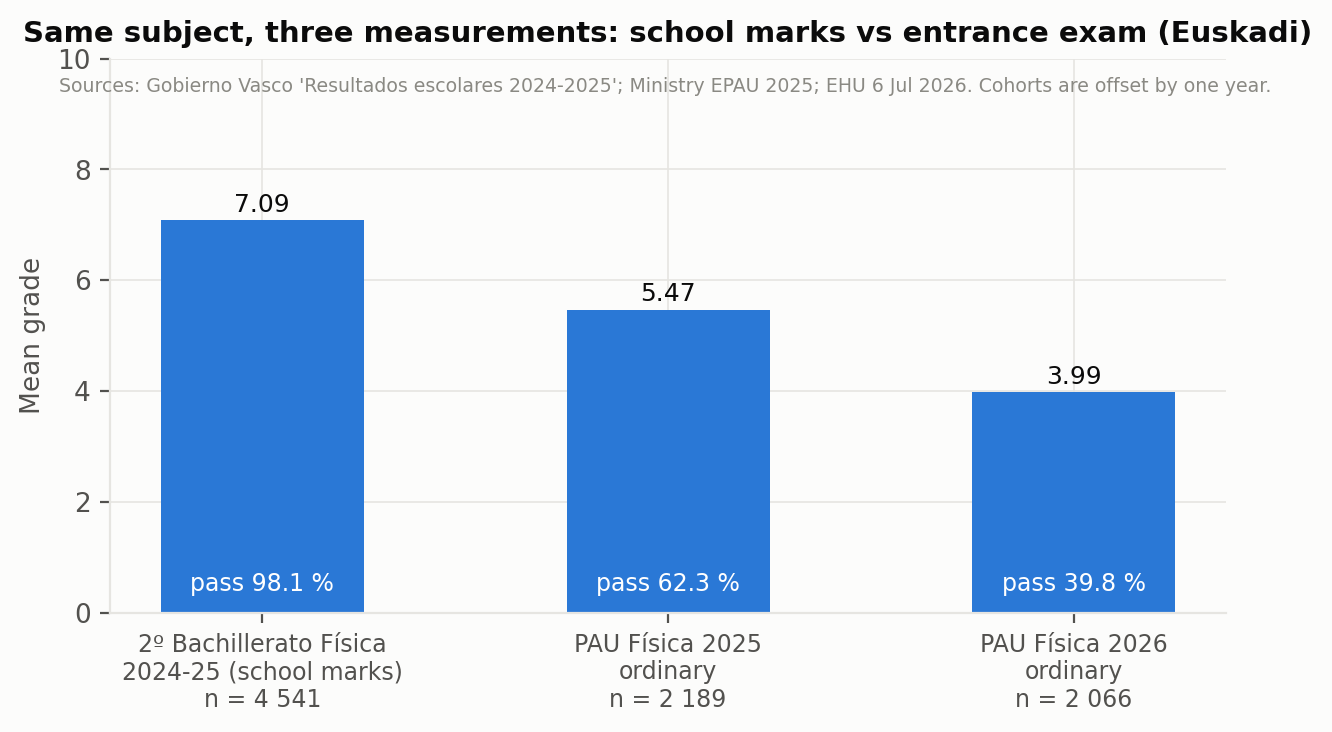
\includegraphics[keepaspectratio]{../plots/fig10_school_vs_pau.png}}

}

\caption{\label{fig-b-school}The same subject measured three times:
school marks of the 2024-25 cohort, PAU Física 2025 and PAU Física 2026.
The cohorts are offset by one year, and the school figure covers all 4
541 students while the PAU figures cover the 2 066--2 189 who sat it.}

\end{figure}%

\textbf{Participation.} Presentation among those enrolled ran 64--84 \%
from 2017 (84.3 \% in 2025); 2026 enrolment is unpublished, so the 5.6
\% fall in candidates cannot be split into enrolment and abstention.
Nationally the Física population grew 30 \% over the decade while
take-up --- the share of PAU candidates sitting Física --- moved only
from 0.222 to 0.240, and within a community take-up is unrelated to the
mean (\(r = -0.10\), \(p = 0.34\)).

\section{The papers}\label{the-papers}

\textbf{One finding in this section was corrected in the seventh round,
and it is the one most often quoted from this briefing.} The Basque 2026
paper is 39 per cent longer to read than the 2025 one, and across the
nine communities length is the strongest single correlate of the change
in the mean (\(r = -0.905\)). Both of those stand. What does not stand
is the account of \emph{why} the Basque paper is long. Splitting both
papers' statements into the narrative and context the competency form
requires, the text that states what to do, and the printed prices, and
normalising per printed statement because 2025 printed seven and 2026
six: \textbf{the narrative is unchanged --- 71 words a statement against
70 --- while the demand text more than doubled, 88 against 181, and the
printed prices went from nothing to 17.} The 2026 criteria itemise each
apartado into sub-items of 0.25, and a paper marked that way has to
print each quantum's demand and each quantum's price. The length is the
cost of the itemisation, not of the competency items
(\href{16-paradigm.qmd}{Ch. 16},
\href{06-interpretation.qmd\#exposure-and-the-third-channel}{Ch. 6}). It
matters for what follows because the two causes are differently
actionable: the competency requirement is imposed from outside and
cannot be declined, while the itemisation is a local decision, taken to
protect candidates, which can be revisited at the cost of the
protection.

Every exercise and option of the eighteen ordinary papers of 2025 and
2026 in the nine communities was coded on the EHU competency criteria
(146 items). A blind second coder repeated the exercise:
\(\kappa = 0.76\) on the competency flag, 0.83--1.00 on drawing, graph
reading, evaluation and explanation, 0.76 on application and 0.70 on the
three-level context code. Every direction of change 2025 → 2026 is
identical under both coders. Separately, the structural claims were
verified against the thirty-two archived PDFs {[}Ch. 11, Ch. 13{]}.

\begin{longtable}[]{@{}
  >{\raggedright\arraybackslash}p{(\linewidth - 8\tabcolsep) * \real{0.2400}}
  >{\raggedleft\arraybackslash}p{(\linewidth - 8\tabcolsep) * \real{0.1200}}
  >{\raggedleft\arraybackslash}p{(\linewidth - 8\tabcolsep) * \real{0.2000}}
  >{\raggedleft\arraybackslash}p{(\linewidth - 8\tabcolsep) * \real{0.2600}}
  >{\raggedleft\arraybackslash}p{(\linewidth - 8\tabcolsep) * \real{0.1800}}@{}}
\caption{Structure and competency content of the eighteen papers {[}Ch.
11{]}.}\label{tbl-b-papers}\tabularnewline
\toprule\noalign{}
\begin{minipage}[b]{\linewidth}\raggedright
Community
\end{minipage} & \begin{minipage}[b]{\linewidth}\raggedleft
Δ mean
\end{minipage} & \begin{minipage}[b]{\linewidth}\raggedleft
Optional \%
\end{minipage} & \begin{minipage}[b]{\linewidth}\raggedleft
Competency-style points, \% of expected
\end{minipage} & \begin{minipage}[b]{\linewidth}\raggedleft
Obligatory competency points
\end{minipage} \\
\midrule\noalign{}
\endfirsthead
\toprule\noalign{}
\begin{minipage}[b]{\linewidth}\raggedright
Community
\end{minipage} & \begin{minipage}[b]{\linewidth}\raggedleft
Δ mean
\end{minipage} & \begin{minipage}[b]{\linewidth}\raggedleft
Optional \%
\end{minipage} & \begin{minipage}[b]{\linewidth}\raggedleft
Competency-style points, \% of expected
\end{minipage} & \begin{minipage}[b]{\linewidth}\raggedleft
Obligatory competency points
\end{minipage} \\
\midrule\noalign{}
\endhead
\bottomrule\noalign{}
\endlastfoot
Asturias & \(+1.13\) & 100 → 100 & 0 → 0 & 0 → 0 \\
Madrid & \(+1.05\) & 75 → 75 & 0 → 0 & 0 → 0 \\
Castilla-La Mancha & \(+0.94\) & 100 → 70 & 0 → 20 & 0 → 2.0 \\
Cataluña & \(+0.80\) & 50 → 50 & 75 → 38 & 5.0 → 0 \\
C. Valenciana & \(+0.51\) & 85 → 80 & 15 → 0 & 1.5 → 0 \\
Andalucía & \(+0.17\) & 60 → 75 & 0 → 0 & 0 → 0 \\
Extremadura & \(-0.82\) & 75 → 75 & 0 → 0 & 0 → 0 \\
Canarias & \(-0.83\) & 100 → 70 & 0 → 0 & 0 → 0 \\
\textbf{País Vasco} & \(\mathbf{-1.48}\) & \textbf{75 → 50} & \textbf{25
→ 62.5} & \textbf{2.5 → 5.0} \\
\end{longtable}

\begin{itemize}
\tightlist
\item
  \textbf{Five of the six rising communities did not increase the
  competency content of their paper.} The sixth, Castilla-La Mancha,
  added one obligatory contextualised item (0 → 20 \%) and rose
  \(+0.94\) --- which is the single most instructive data point in the
  set, because it moved on that axis and on no other.
\item
  \textbf{The Basque paper is the only one that changed genre}, and it
  moved on four axes at once: competency-style content 25 → 62.5 \% of
  expected points, obligatory competency points 2.5 → 5, optionality 75
  → 50 \%, and a granular sub-task format with the highest count of
  marking criteria per item of the eighteen (2.67; Cataluña 2.33).
\item
  \textbf{Cutting choice does not by itself set the direction.} Three
  communities cut optionality by 25 points or more: Castilla-La Mancha
  and Canarias by 30, Euskadi by 25. Two fell; Castilla-La Mancha rose.
\item
  \textbf{Reading load.} Counting statement text only, the Basque paper
  lengthened \textbf{45 \%}, from 1 335 to 1 940 words --- against a
  median of about 1 200 across the eight communities with extractable
  papers, and a range from 899 (Asturias) to 1 628 (Cataluña). Across
  those eight the correlation with the grade change is \(r = -0.905\)
  (\(p = 0.002\)). Three cautions, all material: it leads the
  contextualised-points measure only narrowly (\(-0.86\)), with which it
  is collinear at \(+0.79\); the Basque paper is the leverage point, at
  \(+45\) \% against a next-largest \(+19\) \%; and the hypothesis was
  generated by the coordinator from his own paper, so it is exploratory
  whatever its \(p\)-value.
\end{itemize}

\textbf{Were the nine sitting comparable exams?} Measured against the
three structural criteria as the EHU coordination applies them ---
optionality 50--85 \%, at least 70 \% open response, at least one
obligatory contextualised item --- eight of the nine 2026 papers comply
and one does not: \textbf{Asturias, which rose \(+1.13\), has 100 \%
optionality and no obligatory item at all}. Open response separates
nobody: on the reading made here none of the 146 items uses a closed
format, which is a judgement from the papers rather than a coded
variable. A standardised index of how far each paper moved from its own
2025 predecessor --- optionality, competency marks, substantive context,
contextualised marks --- puts \textbf{Euskadi first at \(+1.76\) SD,
more than a full standard deviation clear of the second}; three
communities moved on no axis but the contextualised share, and none of
the nine is at zero on all four {[}Ch. 11{]}.

The natural conclusion --- that the other communities' 2026 rises are
partly an artefact of papers that did not change --- is the right
direction and it is not established here. What is established is
narrower and still decisive for how the field number should be read:
\textbf{the nine did not sit the same kind of exam, so the field is a
comparison and not a control.} Whether every community was
\emph{required} to move as Euskadi moved cannot be answered from this
study's sources: the text of RD 534/2024 and the Ministry and CRUE
orientations were not retrievable during the data hunt and are not in
the source registry, so no claim of non-compliance by anybody is made or
implied. That gap is data request 9, and it is the difference between
``Euskadi did what was required and others did not'' and ``Euskadi did
more than was required'' --- a compliance question and a design choice
respectively, with very different consequences for 2027.

\textbf{The Basque paper in its own history} {[}Ch. 12{]}. Four formats
since 2010: two whole options A/B to 2019; the COVID ``four-of-eight''
2020--2024; the 2025 paper (four problems of 2.5, one obligatory
competency block, no theory); the 2026 paper (two obligatory competency
exercises, two with a choice). From 2012 to 2024 all 104 theory
questions reproduced verbatim a title from a closed official list of 22,
sent to teachers and correctors with its development guide, worth 40 \%
of the marks. Of the modern-physics problems set in 2010--2024, 14 of 15
were the photoelectric effect. Spherical mirrors were first set in June
2025; standing waves with sound levels and carbon-14 dating in June
2026; a mass spectrometer, obligatory, in July 2026. Marking went from
qualitative rules (2012--2024) to first numerical penalties (2025) to a
printed \(-0.1\) list with symbolic-first, grave errors that may void a
section and 0.25-point sub-items (2026). None of those rules is unique
--- Canarias applies the same list and tightened it the same way, and
fell; Andalucía prints a near-identical one and rose; Valencia requires
symbolic-first and rose. By simulation, choice alone was worth \(+1.24\)
under the 2020--24 format, \(+0.79\) under 2025 and \(+0.53\) under
2026.

\section{The hypotheses, with
verdicts}\label{the-hypotheses-with-verdicts}

\begin{longtable}[]{@{}
  >{\raggedright\arraybackslash}p{(\linewidth - 4\tabcolsep) * \real{0.2400}}
  >{\raggedright\arraybackslash}p{(\linewidth - 4\tabcolsep) * \real{0.1400}}
  >{\raggedright\arraybackslash}p{(\linewidth - 4\tabcolsep) * \real{0.6200}}@{}}
\caption{Ranking: H1b and H2 together at the front and not separable on
published aggregates; H1c plausible behind them; H3 unresolved and
testable; H5 background; H1a a 2025 coincidence; H4 unsupported inside
the PAU; H6 unsupported \href{06-interpretation.qmd}{Ch.
6}.}\label{tbl-b-hyp}\tabularnewline
\toprule\noalign{}
\begin{minipage}[b]{\linewidth}\raggedright
Hypothesis
\end{minipage} & \begin{minipage}[b]{\linewidth}\raggedright
Verdict
\end{minipage} & \begin{minipage}[b]{\linewidth}\raggedright
Grounds
\end{minipage} \\
\midrule\noalign{}
\endfirsthead
\toprule\noalign{}
\begin{minipage}[b]{\linewidth}\raggedright
Hypothesis
\end{minipage} & \begin{minipage}[b]{\linewidth}\raggedright
Verdict
\end{minipage} & \begin{minipage}[b]{\linewidth}\raggedright
Grounds
\end{minipage} \\
\midrule\noalign{}
\endhead
\bottomrule\noalign{}
\endlastfoot
H1a The competency model \textbf{as a national frame} & Describes 2025
at most; does not explain 2026 & Applied in all 17 communities both
years; 14/17 fell in 2025 with Euskadi milder; 6 of 9 rose in 2026. 2025
was also the end of a subject-general plateau and cannot be separated
from it. The only systematic rating of PAU papers' competency
orientation (Universitat Jaume I, six communities, 2015--2025, in
\emph{The Conversation}; primary article not located) places País Vasco
and Cataluña among the \emph{most} competency-oriented before the
reform; Cataluña rose. \\
H1b The competency model \textbf{as the EHU implemented it} &
First-order candidate; the strongest surviving explanation of 2026 & The
frame was national; the implementation was not. On a reform-intensity
index from four independent axes (optionality withdrawn, competency
marks, substantive context, contextualised marks) Euskadi is first of
nine at \(+1.76\), the next community at \(+0.39\). Five of the six
communities that \emph{rose} carry negative indices; \(r = -0.70\),
\(p = 0.035\) across the nine, falling to \(r = -0.40\), \(p = 0.33\)
without Euskadi --- the relation \emph{is} Euskadi. One community
implemented the frame completely and alone. \\
H1c The syllabus reopened, and what the schools were prepared for &
Plausible, unmeasured, not separable from H1b & The narrowing was
\emph{de facto} --- mirrors, standing waves and nuclear decay were never
excluded, only never set, over fifteen years. 2026 reopened them. The
channel is preparation rather than an unavoidable item: in June the new
sub-topics sat in \emph{optional} slots, which bounds the effect and
makes option take-up (request 5) the measurement. Separable from H1b in
principle, not in published aggregates: both are properties of one paper
in one year and both displace the whole distribution. \\
H2 The 2026 Basque paper \textbf{as a format} --- length, optionality,
genre & Consistent with everything; first-order variable & Set apart
from H1b: reading load \(+45\) \%, to about 1 430 words of statement;
choice halved, two of four problems carrying none (\(-0.26\) by
simulation); the only paper in the set that changed genre. The whole
distribution displaced; damage confined to Física and Matemáticas II;
the Catalan mirror image. \\
H3 Tribunals marked more severely & Possible, unmeasured, acknowledged
by EHU & The rector reported ``significant variation between panels'' in
Física; the 6 July deck gave tribunal ranges for three other subjects
and not for Física. The whole-cohort shape says severity, if present,
was general rather than confined to a few panels. Only the tribunal
table settles it. \\
H4 A weaker or differently composed cohort & Weak inside the PAU; real
outside it & Presentation fell 5.6 \%; the same students held Química
and Biología; take-up flat; the Canarian cohorts sit on the locus. But
PISA shows a decade-long Basque decline that the PAU sees only in Física
and only from 2025. \\
H5 Weighting rules make Física dispensable & Plausible slow driver, not
a 2026 trigger & The Canarian coordinators' hypothesis for their own
decline; fits a slow erosion better than a 1.5-point fall. \\
H6 Language or network bias & No evidence either way for Física & Only
the Euskara II bias analysis was run; the 2010--2022 differences are
small and of both signs. \\
\end{longtable}

\section{PISA 2025 and the 2027
estimate}\label{pisa-2025-and-the-2027-estimate}

PISA is the one instrument that measures these students and is marked
outside the Basque system. A standing Basque advantage in science became
a deficit a decade ago: \(+6.2\), \(+6.4\) and \(+9.2\) points above
Spain in 2006, 2009 and 2012; then a fall of 22.6 points between 2012
and 2015 while Spain fell 3.7, and no recovery. \textbf{PISA 2025,
published on 8 September 2026, is the cohort that sits the PAU in 2027
and is the weakest recorded}: Basque science 458.5 against Spain 477.1
and the OECD 481.9, a gap of \(-18.6\) (one standard error 4.7), with
the Basque share at proficiency levels 5--6 falling from 3.32 \% to 1.83
\%.

\begin{figure}[htbp]

\centering{

\pandocbounded{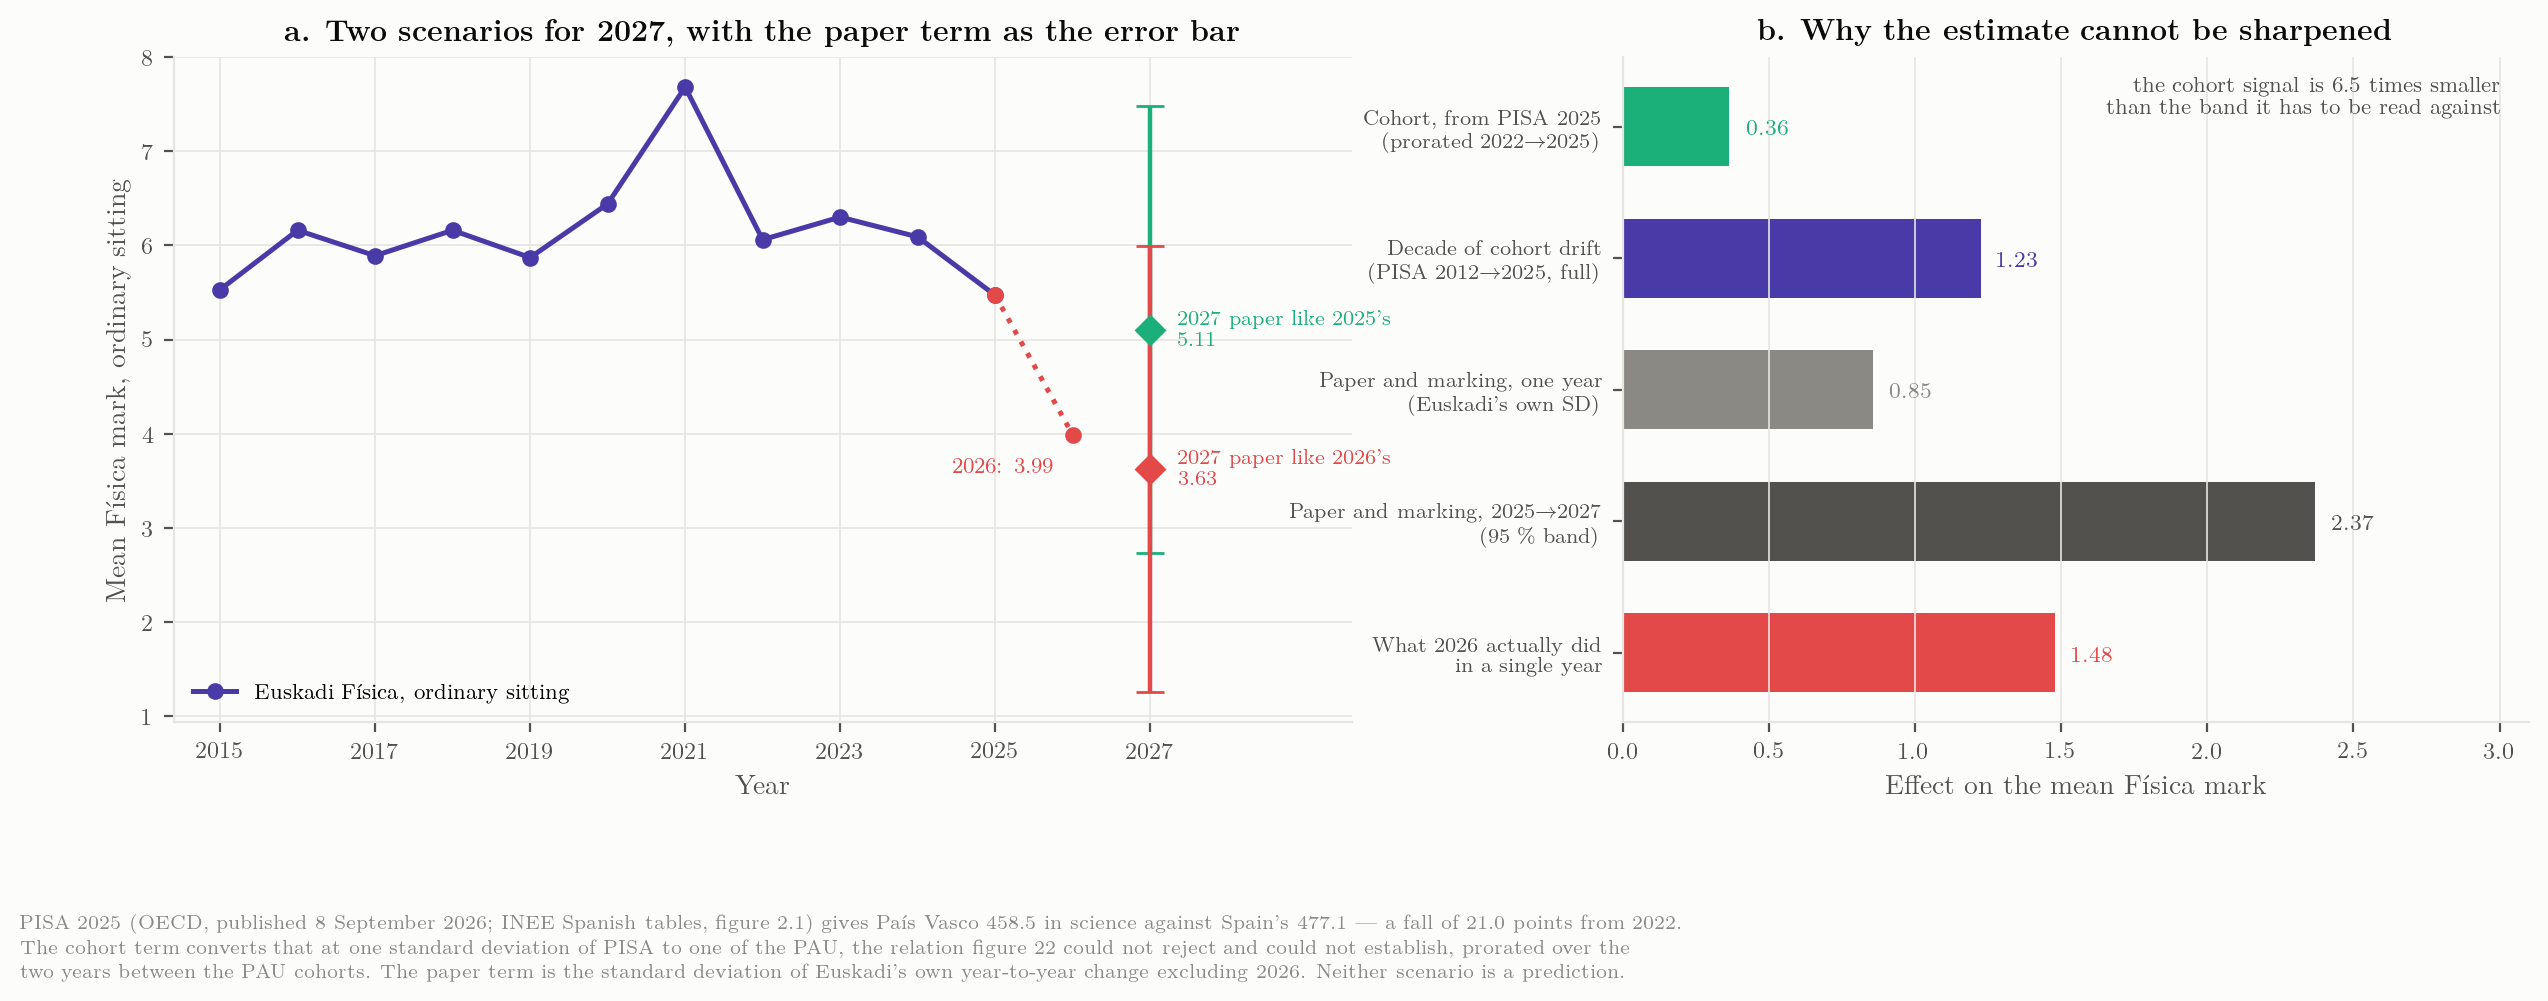
\includegraphics[keepaspectratio]{../plots/fig23_pau2027.png}}

}

\caption{\label{fig-b-2027}\textbf{a} --- the Basque series with two
scenarios for 2027; the bar is the year-to-year term, not a prediction
interval. \textbf{b} --- the one estimated cohort term against the
dispersion it must be read through, and against what 2026 actually did.}

\end{figure}%

Converting that into a PAU estimate is arithmetic, and the arithmetic is
the finding. The Basque PISA fall of 21 points is 0.23 of a student
standard deviation; transferred one-for-one to the PAU and prorated over
the two years between the 2025 and 2027 cohorts it is a \textbf{cohort
term of \(-0.36\) marks}, or \(-0.18\) measured from 2026. Three
conventions sit inside that number and should travel with it: the
transfer is one-for-one because nothing in the data rejects it; the PAU
standard deviation of 2.343 comes from the Comunitat Valenciana's
published figures, the only ones available; and the PISA standard
deviation of about 90 is Spain's.

\begin{longtable}[]{@{}lrr@{}}
\caption{Two scenarios for 2027
(modelled).}\label{tbl-b-2027}\tabularnewline
\toprule\noalign{}
If the 2027 paper resembles & Cohort term & Central estimate \\
\midrule\noalign{}
\endfirsthead
\toprule\noalign{}
If the 2027 paper resembles & Cohort term & Central estimate \\
\midrule\noalign{}
\endhead
\bottomrule\noalign{}
\endlastfoot
the 2025 paper & \(-0.36\) & \textbf{5.11} \\
the 2026 paper & \(-0.18\) & \textbf{3.81} \\
\end{longtable}

\textbf{PAU 2027 is not something PISA predicts; it is something the
2027 paper and its marking decide.} The two scenarios differ by 1.3
marks; the cohort contributes a third of a mark. Two practical uses:
assume an intake slightly weaker than 2025's and considerably weaker
than the decade's average, and set the paper with that in mind rather
than against a remembered cohort; and when the 2027 result arrives,
about \(-0.36\) is the part that should not be attributed to the paper.

\subsection{Can a rate of decay be
projected?}\label{can-a-rate-of-decay-be-projected}

The coordination has asked whether the cohort decline can be turned into
a \emph{rate}, so that a PAU year could be anticipated before it is sat.
Four answers, in order.

\begin{figure}[htbp]

\centering{

\pandocbounded{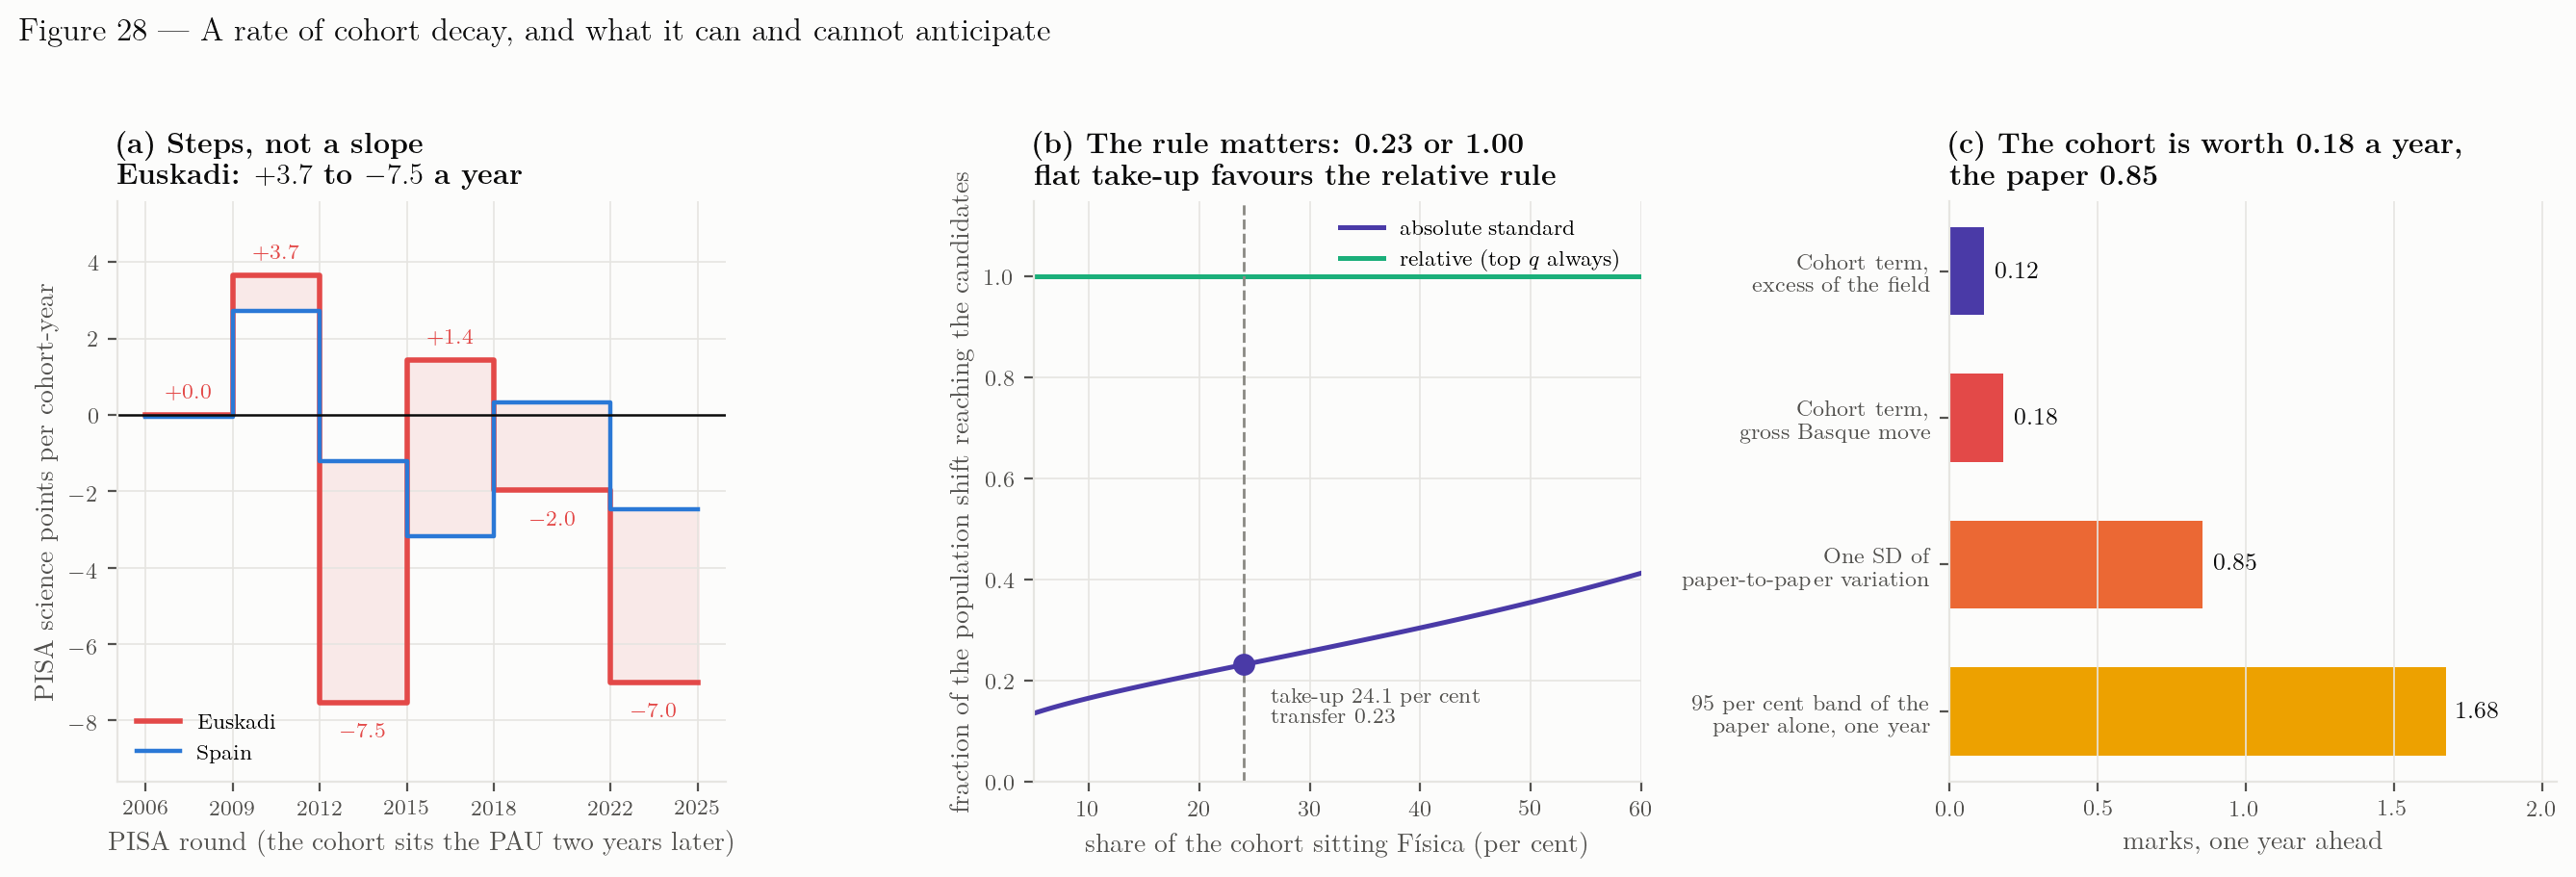
\includegraphics[keepaspectratio]{../plots/fig28_cohort_rate.png}}

}

\caption{\label{fig-b-cohortrate}\textbf{a} --- the change in PISA
science per cohort-year between consecutive rounds. \textbf{b} --- how
much of a shift in the whole population reaches a self-selected upper
fraction, under a fixed ability bar and under a fixed share. \textbf{c}
--- what the cohort term is worth against what the paper is worth, one
year out.}

\end{figure}%

\textbf{The rate is not a slope.} Between consecutive PISA rounds the
Basque change per cohort-year runs \(+0.01\), \(+3.65\), \(-7.53\),
\(+1.44\), \(-1.97\), \(-6.99\) points --- a spread of 11.2 points a
year around a mean of \(-1.90\). Two of the six intervals carry almost
the whole decline and three are flat or positive. A line fitted through
them would have a slope, and quoting it would put an honest interval
around the wrong model. The cohort that sat PAU 2026 was fifteen in
spring 2024, between rounds, so PISA never measured it at all: the
cohort term used above interpolates, and assumes the fall was spread
evenly over three cohorts.

\textbf{A constant within-cohort degradation is invisible, and that is
the right answer rather than a failure.} Write the PAU mean as
\(s[A(c,15) + G(c)] + \mathrm{sel}(c) + \mathrm{paper}(y) + \mathrm{marking}(y)\),
with \(G\) the gain or loss over the three school years. PISA delivers
\(A(c,15)\) and nothing about \(G\), which enters every year-to-year
difference alongside the paper term --- the largest and least measured
term in the dossier. A \(G\) that is \emph{constant} cancels in every
difference: it is invisible precisely because it is irrelevant to the
question the office faces, which is why one year differs from the next.
A \(G\) that is \emph{changing} would matter, and would show as the PAU
falling faster than PISA for matched cohorts. It falls more slowly
(\(-0.157\) against \(-0.245\) SD per decade in Euskadi, difference
\(p = 0.67\)) --- no support for acceleration, and at four to six points
per series no refutation either.

\textbf{The motivated/unmotivated split is real, and in 2026 it runs the
wrong way for dilution.} If more candidates sit Física without needing
the mark, the mean falls with nobody's ability changing. In 2026 it
cannot have happened: 2 066 sat Física against 2 189 in 2025, 5.6 \%
fewer. On the assumption most favourable to the dilution story --- that
the ones who stayed away were the weakest --- the 2026 group should have
scored \textbf{0.29 marks higher} on an unchanged paper. The composition
change is a credit against the fall, not a part of it. (2025 is the
opposite case, 22.4 \% more candidates with a mean 0.62 lower; and the
budget assigns 2025 almost wholly to the national component in any
case.)

\textbf{How much of a population shift reaches the candidates} depends
on how selection works, and the two natural rules differ by a factor of
four: 0.23 of the shift under a fixed ability bar, exactly 1.00 under a
fixed share. The evidence points at the second --- a falling population
under a fixed bar should produce falling take-up, and take-up instead
drifts slightly up (0.222 in 2015 to 0.240 in 2025, \(r = -0.096\),
\(p = 0.34\)) --- and independently, the Basque PISA fall is a location
move rather than a collapse of the top: the level 5--6 share went 3.32
\% → 1.83 \% where a uniform shift of the whole distribution predicts
1.92 \%, a discrepancy of just under five per cent of the predicted
share. So the one-for-one conversion used above is defensible, but it is
the \emph{top} of the range: the cohort term is an upper bound in
magnitude and could be as small as \(-0.03\) a year.

\textbf{What follows for practice.} A cohort projection is real, is
worth about a fifth of a mark a year, and is swamped by the choice of
paper: one standard deviation of paper-to-paper variation is 0.85,
nearly five times the cohort term, and the 95 \% band one year out is
1.68, roughly nine times it. It belongs in the office's expectations and
not in its targets. If the 2027 mean comes in half a point below 2026,
nothing about the cohort will have been demonstrated; if two points
above, nothing will have been refuted.

\textbf{What would give a rate} is not PISA, which measures every three
years and stops at fifteen. It is a yearly census measure of Basque
fifteen-year-olds, bracketed at the other end by the school marks of the
same cohort at eighteen --- which EHU already holds paired with the PAU
mark for every candidate, and which this study has for one year only
(7.09 against 5.47 in 2025). That pairing over several cohorts is the
design that separates a cohort arriving weaker from a cohort being
taught and examined differently. It is \textbf{data request 8}.

\section{What the evidence does not
establish}\label{what-the-evidence-does-not-establish}

The dossier was audited twice, on 19 and 20 September: every script
re-run from the raw sources, every number recomputed independently by
readers working only from the files, the exam papers re-read as PDFs,
all 25 figures checked against their data, and the reasoning read step
by step. The second audit corrected the first, which had reported three
corrections it had not applied. Everything above is the audited version
{[}Ch. 13{]}.

What remains genuinely open:

\begin{itemize}
\tightlist
\item
  \textbf{H2 against H3 cannot be separated from published data.} A
  harder paper and uniformly stricter marking leave the same
  whole-cohort signature.
\item
  \textbf{Three quarters of the Basque-specific fall is unattributed},
  among four named candidates that the published aggregates cannot prise
  apart.
\item
  \textbf{The 2026 Basque distribution is modelled.} Only the observed
  histogram would say whether it, like the Canarian cohorts, moved
  without reshaping.
\item
  \textbf{Whether 2024 and 2026 are one mechanism or two} is undecided.
  A compression at the top in 2024 and a collapse of the level in 2026
  are compatible with a single slow change in what the marking rewards,
  and equally compatible with two unrelated events.
\item
  \textbf{The Euskadi-common \(-1.18\) has no candidate explanation at
  all.} It is larger than the Física-specific term, it moved Matemáticas
  II further than Física, and nothing in this dossier isolates it. It is
  not the Física paper, because Química and Biología sat the same
  tribunals and did not follow.
\item
  \textbf{The two versions of the severity hypothesis are not
  separated.} The subject pattern excludes a general effect as the main
  cause and is consistent with a numerical-deduction effect; consistency
  over eight subjects in one year is not a test, and the deduction tally
  is.
\item
  \textbf{The within-cohort term cannot be identified} from PISA and the
  PAU together, at any sample size, because it enters every difference
  alongside the paper term. Only paired school and PAU marks over
  several cohorts would bound it.
\item
  \textbf{Several figures are press-sourced} (Extremadura 5.27;
  Asturias's headline and subject values; the EHU July figures; the
  Catalan revision requests) and should be confirmed before being quoted
  onward.
\end{itemize}

\section{Data to request, and what each would
separate}\label{data-to-request-and-what-each-would-separate}

Ordered by how much of the unattributed \(-1.33\) each would resolve,
not by how easy it is to obtain. Items 3, 8 and 9 are new since the
first version of this briefing.

\begin{enumerate}
\def\labelenumi{\arabic{enumi}.}
\tightlist
\item
  \textbf{Sub-task marks for a stratified sample of 2026 scripts} (say
  300, across tribunals): the mean and distribution of marks on each
  numbered sub-task of each exercise and option. \emph{Separates all
  four} unattributed components at once, because each leaves a different
  signature --- marks lost in the obligatory competency exercises rather
  than the options (content); in the explain-and-evaluate sub-tasks
  rather than the calculations (genre); through accumulated \(-0.1\)
  penalties and voided sections (marking); only among those who chose
  the new options (exposure).
\item
  \textbf{Física by tribunal, 2025 and 2026}: \(n_j\), \(\bar{x}_j\),
  \(s_j\) and the school composition of each tribunal's scripts. EHU
  computed this and published the equivalent for three other subjects.
  \emph{Separates} tribunal severity, and shows whether what is visible
  in 2026 was building in 2025.
\item
  \textbf{The deduction tally, 2025 and 2026, for Física, Matemáticas
  II, Lengua Castellana and Euskara II}: how many scripts lost the 0.2
  linguistic component, and how many \(-0.10\) minor-error deductions
  were applied per script, by type. \emph{Separates} general marking
  severity from the quantitative-specific kind. \textbf{This is the
  cheapest decisive request on the list}: it collects nothing new, the
  four subjects are already marked, and the comparison the coordination
  wants falls out of two cross-tabulations. If one item can be obtained
  quickly and from inside the university, it is this one.
\item
  \textbf{The full Física histogram for 2024, 2025 and 2026}, in
  one-point bands with the zero and ten counts. \emph{Separates}
  location from shape in 2026 --- the classification this study could
  not make --- and tests the 2024 compression directly.
\item
  \textbf{Option take-up in 2026}: how many chose each of 3a/3b and
  4a/4b, and the mean of each. \emph{Separates} syllabus exposure from
  paper difficulty, and measures the realised choice premium against the
  simulated \(-0.26\).
\item
  \textbf{July 2026 Física}: presented, passed, mean. \emph{Separates}
  whether the June pitch was that paper or the 2026 marking.
\item
  \textbf{Revision statistics for Física 2026}. \emph{Separates} marking
  severity weakly but cheaply.
\item
  \textbf{School mark and PAU mark, paired, for every Física candidate
  of the last five cohorts}, with sex, language and territory, and the
  enrolment figures published until 2022. \emph{Separates} two things:
  who sat the exam, which is currently bounded rather than measured;
  and, over cohorts, the within-cohort term \(G\) --- the only
  instrument available for it, since the school mark and the PAU mark
  are two measurements of the same students weeks apart against two
  different standards.
\item
  \textbf{The other eight communities' 2026 papers and marking criteria
  with their published means}, and the text that fixes the structural
  criteria nationally, if it exists. \emph{Separates} nothing inside
  Euskadi, but decides how much weight the field comparison can carry.
  Until it is settled, the \(-1.65\) is a comparison with communities
  that did something different, not with a control group.
\item
  \textbf{The record of the correctors' meeting held before the 2026
  sitting}: agenda, attendance and the criteria document circulated.
  \emph{Separates} nothing by itself, but it is what turns the account
  of the regime change from testimony into record. It costs nothing to
  retrieve.
\item
  \textbf{The 2026 grade-band table for Física} --- the shares in
  \([0,5)\), \([5,6)\), \([6,7)\), \([7,8)\), \([8,9)\) and \([9,10]\),
  the same table published every year through 2025. \emph{Separates} how
  the penalties were spread across candidates, and with it how much of
  the fall the marking can be held to account for. Seven readings of the
  same regime, each refitted on its own parameters, match all four
  published figures and differ on the share at or above nine by a factor
  of twenty-three --- 0.3 \% if the penalties fell evenly on everybody,
  6.1 \% if they concentrated on the weakest --- which is the difference
  between the marking accounting for 87 \% of the Física-specific fall
  and 59 \% of it. \textbf{This is the cheapest request on the list}:
  the table is a by-product of a tabulation already run and it was
  routine until last year. The \(2.09\) \% this dossier quotes for that
  band is its own smooth-curve extrapolation and is labelled modelled
  throughout; it is not a substitute.
\end{enumerate}

\textbf{If request 1 is refused as too laborious}, the substitute is a
blind re-marking of a stratified sample of 2026 scripts by a second
panel: it costs marking time instead of clerical time and it answers
requests 1 and 2 together. \textbf{If request 2 is refused}, requests 4
and 7 together give a weaker version of the same answer. Nothing
substitutes for all three. \textbf{Request 3 is the exception to the
ordering} --- it is decisive for one component and obtainable within
days, so it should be made first whatever else is agreed.
\textbf{Request 11 is the second exception}, for the same reason and at
even lower cost: it is one table that already exists, and it settles a
question on which two readings of the same marking regime differ by a
factor of twenty-three.

\section{Design levers for 2027, ordered by evidence and
cost}\label{design-levers-for-2027-ordered-by-evidence-and-cost}

None of these is a recommendation to abandon the competency model, which
the evidence does not indict: the most competency-oriented papers in
Spain before the reform --- Cataluña's and Euskadi's own, on the one
systematic rating available --- sit in communities that went opposite
ways in 2026, and Cataluña's decade of fully contextualised papers is in
the one that rose.

\begin{enumerate}
\def\labelenumi{\arabic{enumi}.}
\tightlist
\item
  \textbf{Record the paper's parameters before the sitting} and read the
  result against them: statement length per exercise, competency share,
  optional share, penalty rules, topics examined, and the PISA cohort
  term (\(-0.36\)). Costs nothing, requires no new belief, and is what
  makes 2027 interpretable whatever it produces. \emph{Evidence: not
  needed --- this is measurement, not a hypothesis.}
\item
  \textbf{Treat Física and Matemáticas II as one problem.} More than
  half of the Basque-specific fall is a term the two share, and neither
  \emph{ponencia} can see it from inside its own subject: Matemáticas II
  fell 1.67 on the same cohort and the same tribunals. A joint reading
  of the two subjects' 2026 results --- and, when it arrives, of the
  deduction tally for both --- is the cheapest way to find out whether
  the shared term is the cohort, the marking regime, or the simultaneous
  format change in two quantitative subjects. \emph{Evidence: the exact
  subject split, which is arithmetic rather than a model; what the
  shared term} is \emph{remains open.}
\item
  \textbf{Keep a monitoring set}: mean, pass rate, band shares, and each
  subject's mean against its own 2015--2019 norm, computed per tribunal.
  The subject-against-own-norm comparison is what showed that Física
  alone was below norm in 2025; the band shares are what would have
  shown the 2024 compression at the time. \emph{Evidence: strong ---
  both findings came from these statistics.}
\item
  \textbf{Set and record a target statement length --- and decide where
  the words come from, which is a separate decision and the harder one.}
  The 2026 statement was 45 \% longer than 2025's and the longest of the
  sixteen papers whose text could be extracted; the 2026 median across
  those is about 1 200 words and the 2025 Basque paper was 1 335. A
  target near the Basque paper's own 2025 length --- say 1 300--1 400
  words for the whole statement --- is the defensible starting band, and
  it is a bookkeeping target rather than a finding. \textbf{What the
  seventh round adds is that the slack is not where this briefing
  previously implied it was.} Per printed statement the contextual
  narrative is already at 70 words and has not grown since 2025; the
  growth is 93 words a statement of demand text and 17 of printed
  prices, both of which exist because the marking is itemised into
  quanta of 0.25 and printed on the paper. Four routes, three of which
  this dossier can price in words and none in marks: compress the
  narrative (there is not 470 words of slack in it); flatten two levels
  of demand back to one (cheapest, and it returns partial credit to the
  corrector's discretion); itemise in the criteria as now but print only
  the apartado and its total (the only route that separates the reading
  cost from the protection, and nobody has tested whether candidates use
  the printed weights); or leave the length alone and cap the deductions
  instead, which is item 8. \emph{Evidence: the strongest
  cross-community association in the study by a short head
  (\(r = -0.905\) against \(-0.86\) for contextualised points), and the
  weakest causally --- it is post-hoc, collinear with competency
  content, and leveraged by the Basque paper itself. The decomposition
  of the statement, by contrast, is a direct measurement of the Basque
  papers themselves and is corroborated independently by the
  coordination's own reconstruction, which prices the itemisation step
  at 66 words on one problem.}
\item
  \textbf{Restore a choice inside the obligatory competency exercises}
  --- two contexts, the same \emph{saber básico} --- rather than
  restoring optionality elsewhere. The two simulated formats differ by
  0.26 of expected mark; a third format with a choice inside the
  obligatory exercises was not simulated, so that figure is an
  indication of the size of the lever and not a prediction for it.
  \emph{Evidence: a simulation of the actual formats, plus the
  coincidence of the most generous choice rule with the highest means in
  the series. Note that cutting choice did not set the direction:
  Castilla-La Mancha cut it by more and rose.}
\item
  \textbf{Publish which \emph{saberes} can carry a problem in 2027, with
  model items.} For fifteen years modern physics meant the photoelectric
  effect; in 2026 three topics were examined for the first time. Opening
  the syllabus is legitimate; opening it unannounced in the same year as
  everything else is not what the record recommends. \emph{Evidence: the
  inventory of 146 problems, plus the coordinator's account of the
  restriction.}
\item
  \textbf{Pace the deployment: change one axis a year and announce it.}
  The one paper that moved on four axes at once fell furthest; the 2025
  break taken alone was absorbed better than the Spanish average.
  \emph{Evidence: n = 1 --- and the count of axes is four on this
  study's own coding, three on an earlier one --- which is why it sits
  seventh rather than first despite being the most plausible
  recommendation in the list. 2028 is the year the model is to be fully
  deployed.}
\item
  \textbf{Decide the marking questions explicitly, and count the
  deductions first.} The tally of request 3 comes before any decision
  here, because it says whether the second year of the criteria was in
  fact stricter and whether it was stricter in the same way for a
  physics script as for a language script. Then three questions the
  seventh round makes concrete. \textbf{Whether the \(-0.10\) deductions
  should stay uncapped}, when the linguistic penalties in the same
  criteria are capped at 1.00 and every other community that specifies a
  cap applies one to the numerical deductions too --- Andalucía at
  \(-0.25\) per apartado, Extremadura at 1.00, Canarias at 20 \% of the
  section until it removed the cap in 2026. \textbf{Whether a penalty of
  \(0.10\) belongs in a scheme built on a quantum of \(0.25\)}, since
  one deduction takes a sub-item to 0.15 and no script is on the grid
  after the first. And \textbf{whether the deductions should fall on
  half the paper}: only 14 to 19 of a script's 27 to 32 sub-items can
  attract a unit, prefix or rounding error, so the uncapped penalties
  land on the numerical part --- which is precisely the part the
  itemisation was introduced to make forgiving. Then also: whether
  grave-error clauses that void a whole section are applied uniformly
  across tribunals (the tribunal table will show it), and whether
  borderline rounding is wanted --- at the ULL its thinning was worth
  about 5.6 points of pass rate, while the ULPGC shows no such bunching
  at all, and whether EHU rounds at the threshold is not published.
  \emph{Evidence: no single rule is indicted; their joint introduction
  in one year is.}
\item
  \textbf{Calibrate against a target distribution and pre-test.} The
  Ministry cube gives a full band distribution for every subject,
  community and year; the 2017--2024 Basque structure outside the COVID
  peak is \([0,5)\) ≈ 30 \%, \([9,10]\) ≈ 16 \%. A pre-test on 40--60
  Bachillerato students from two or three centres, sat under exam
  conditions on a paper that will not be used, gives a usable mean to
  within about half a point and a clear read on whether the paper can be
  finished. \emph{Evidence: the practice exists informally in other
  communities' ponencias; its effect here is untested.}
\item
  \textbf{Second marking and external review} of the paper before the
  sitting, on the Galician 2027 model (peer review of papers, double
  marking), with Rasch equating of tribunals as the statistical
  complement. \emph{Evidence: one Galician announcement and one
  methodological literature; no effect measured in this data.}
\item
  \textbf{Timetable.} Física sits in the last slot of the science day in
  Canarias, whose coordinators name it as a factor; the Basque timetable
  is a free parameter. \emph{Evidence: one set of minutes from another
  community.}
\end{enumerate}

\textbf{What this needs from the office.} Items 1 and 3 are decisions
for the coordination alone and can be taken now. Item 2 needs the
office, because no single \emph{ponencia} can convene it. Items 4 to 8
belong in the 2027 coordination instructions and therefore have to be
settled before those instructions go to schools --- which, on the 2026
calendar, means before the end of the autumn term. Items 9 to 11 need
the admissions office: a pre-test needs permission and centres, double
marking needs budget, and the timetable is set centrally. And the data
requests are the office's to make of EHU; nothing in the first three
levers is blocked by them, but the choice between remedies in items 4 to
8 is --- and request 3, the deduction tally, is both the cheapest and
the one that would most change which of those remedies is right.

\section{Sources and reproducibility}\label{sources-and-reproducibility}

The dossier archives 166 source files with their hashes: the EHU decks
and annual reports, the Ministry EPAU cubes 2015--2025, the Basque
Inspectorate's school results, the transcribed dashboards of ULL, ULPGC
and UCLM (recorded as read, without file hashes), the 2025--2026 papers
of nine communities with the corrector documents that exist for seven of
them, the complete EHU archive 2010--2026, the official theory list, and
the INEE PISA tables 2006--2025. Every number in this briefing is
produced by a script in \texttt{scripts/} from those files and can be
regenerated with one command; the two audits and their layer reports are
in \texttt{logs/}. The figures are reproduced as generated, with English
labels.




\end{document}
